\documentclass[a4paper,authoryear,review]{elsarticle}

\usepackage[utf8]{inputenc}
\usepackage{amssymb}
\usepackage{lineno}
\usepackage{url}
\usepackage{hyperref}
\usepackage{caption}
\usepackage{subcaption}
\usepackage{graphicx}
\usepackage{adjustbox}
\usepackage{epstopdf}
\usepackage{gensymb}
\usepackage{xcolor,colortbl}
% \usepackage[table,xcdraw]{xcolor}
% If you use beamer only pass "xcolor=table" option, i.e. \documentclass[xcolor=table]{beamer}
\usepackage[normalem]{ulem}
\useunder{\uline}{\ul}{}
%TODO: remover
\DeclareUnicodeCharacter{0301}{\'{e}}
\hypersetup{unicode=true,
           colorlinks=true,
           linkcolor=blue,
           citecolor=blue,
           filecolor=red,
           urlcolor=blue,
           breaklinks=true
           }

\journal{Journal of Computers and Electronics in Agriculture}

%% `Elsevier LaTeX' style
\bibliographystyle{elsarticle-harv}
%%%%%%%%%%%%%%%%%%%%%%%

\begin{document}

\begin{frontmatter}

\title{Deep Learning for 2D grapevine bud detection}

\author[utn]{Wenceslao Villegas Marset\corref{cor1}}
\ead{diego.villegas@alumnos.frm.utn.edu.ar}

\author[utn]{Diego Sebastián Pérez}
\ead{sebastian.perez@frm.utn.edu.ar}

\author[utn]{Carlos Ariel Diaz}
\ead{carlos.diaz@frm.utn.edu.ar}

\author[utn,conicet]{Facundo Bromberg}
\ead{fbromberg@frm.utn.edu.ar}

\address[utn]{Universidad Tecnológica Nacional, Facultad Regional Mendoza, Grupo de Inteligencia Artificial DHARMa, Dpto. de Sistemas de la Información. Rodríguez 273, CP 5500, Mendoza, Argentina.}

\address[conicet]{Consejo Nacional de Investigaciones Científicas y Técnicas (CONICET).}

\cortext[cor1]{Corresponding author}

\begin{abstract}
%Intro / Motivación - Desafío - Técnicas - Resultados 
Visual inspection is a task necessary to measure relevant variables in viticulture and is susceptible to being automated with computer vision methods. Bud detection is central for various of these tasks such as: measurement of buds’ sunlight exposure, autonomous pruning, bud counting, type-of-bud classification, bud geometric characterization, internode length, and bud development stage, among others. This paper presents a method for grapevine bud detection based on a \emph{Fully Convolutional Networks Mobile-Net} architecture. To validate its performance we compare it on the detection task with the known state-of-the-art method for bud detection, showing improvements over three of the aspects of detection: \emph{segmentation}, \emph{correspondence identification} and \emph{localization}. In its best version of configuration parameters, our approach showed a detection precision of $95.6\%$, detection recall of $93.6\%$, a mean Dice coefficient of $89.1\%$ for correct detection (i.e., detections whose mask overlaps the true bud), with small and nearby false alarms (i.e., detections not overlapping the true bud) as shown by a mean pixel area of only $8\%$ the area of a true bud,  and a distance (between mass centers) of $1.1$ true bud diameters. The paper concludes with a discussion on the  advantages of our approach for real-world applications.
\end{abstract}

\begin{keyword}
Computer vision \sep Fully Convolutional Network \sep Grapevine bud detection \sep Precision viticulture
\end{keyword}

\end{frontmatter}

\linenumbers

%#######################################################################

\section{Introduction} 

% Problem: detection, Solution: FCN
In this work we propose a solution for the autonomous detection of grapevine buds within 2D images of vineyards captured in natural field conditions. Our proposed approach is based on \emph{Fully Convolutional Networks} (FCN) \citep{long2015fully, shelhamer2017fully}, a kind of deep learning model specific for computer vision applications. Our solution adds in the historical quest for more and better quality information about different vineyard processes that impact on the productivity of grapevines and quality of their grapes. 

% ¿why bud related variables are important?  fertility
% ¿why fertility is important? main goal of grapevine producers is to estimate and the guarantee the grapevine production.
%
For years viticulturists have been producing models of the most relevant plant processes (i.e. fruit quality and yield, soil profiling, vine health), and they have been recollecting a diverse collection of information for feeding these models. Better and more efficient measuring procedures resulted in more information with its corresponding impact on the quality of models’ outcomes, while inspiring researchers to push the boundaries for producing more sophisticated models. Such information consists of a large set of variables for assessing different aspects of the parts of the plant involved in these processes: trunks, leaves, berries, buds, shoots, flowers, bunches, canes. The list is long, with examples of these variables being berry maturity, number, weight, size and volume; cluster compactness, morphology such as length, width, size, and elongation, as well as cluster volume, number and weight; buds burst, number and size; flowers number; leaf area; shoot length; pruning weight; canopy density; among others \citep{awriNDmanual1, awriNDmanual3}),
%
Nowadays technology is pushing once again the possibilities in the quality and throughput of these measurements, with digital and autonomous measurement procedures that improve over manual measurement procedures. The discipline is experiencing a transition, with many of its variables still being measured manually through visual inspection, resulting in large labor costs that limits the measurement campaigns to only small samples of data, that even with the use of statistical inference or spatial interpolation techniques impose a bound in the quality of the outcomes \citep{whelan1996spatial}. 
%
In some cases this is exacerbated by the need of experts for a proper measurement, such as the case of variables associated to the phenological stages of the plant such as bud swelling, bud burst, inflorescence, flowering, veraison, ripening of berries, among others \citep{lorenz1995growth}; or by measurement procedure that requires the destruction of the part of the plant being measured, preventing any tracking of the variables overtime. Such is the case for the measurement of leaves area, bunch weight, berry weight and pruning weight \citep{kliewer2005leaf}. 

%
Precision viticulture in general \citep{bramley2009lessons}, and computer vision algorithms in particular, has been growing in the last couple of decades, mainly for their potential for mitigating these limitations \citep{seng2018computer, matese2015technology}. These algorithms come along with a promise of an unprecedented boost in the production of vineyard information, with much expectations not only on possible improvements in the quality of the models’ outcomes, but in its potential to produce better models by feeding all this information to big data algorithms. 

%
In this work we contributed to this general endeavour with an algorithm for measuring variables related to one specific part of the plant: the bud; an organ of major importance for being the grow point of the fruits, containing within all the productive potential of the plant \citep{may2000bud}. Our contribution of  autonomous bud detection not only enables the autonomous measurement of all bud related variables currently measured by agronomists (see Table$\sim$\ref{tab:Tabla1} for a non-exhaustive list of bud related variables); but has the potential to enable the measurement of novel, yet important variable  that are currently impossible to be measured manually. One example is the total sunlight captured by the buds, that depends on the manually unfeasible task of determining the exact location of buds in 3D space.  Although the present work focuses on 2D detection, it could be easily upgraded to 3D by, for instance, integrating the 2D detection in the workflow proposed by \cite{diaz2018grapevine} (c.f. Section$\sim$\ref{sec:related} for some more details on this workflow).

%
Table$\sim$\ref{tab:Tabla1} shows a non-exhaustive list of the most important bud related variables currently measured by vineyard managers \citep{sanchez2005bud, noyce2016basis, collins2020effects}, accompanied by an assessment of the extent to which detection contributes in their measurement. The right-most column indicates what information beyond detection  is necessary to complete the measurement, while the middle columns labeled (i), (ii), and (iii) indicate what specific aspects of the detection are required for that variable: (i) whether it requires a good  \emph{segmentation}, i.e., the discrimination of which pixels in the scene correspond to buds and which ones correspond to the background (no-bud); ii) a good \emph{correspondence identification}, i.e., discrimination of bud pixels as belonging to different buds; or (iii) a good \emph{localization}, i.e., the localization of the bud within the scene; respectively.
%
For instance, tomemos por caso la variable \emph{buds number}. De ser posible identificar correctamente las correspondencias, the buds number coincide directamente con el conteo de detecciones. Por el contrario, para \emph{type-of-bud classification}, además de identificar correspondencias, la segmentación de la parte de la imagen perteneciente a la yema es necesaria para poder así alimentar a un clasificador con la información visual relevante, minimizando el ruido producto de pixeles del background. Por último, para medir la \emph{incidence of sunlight on the bud}, no es necesaria la segmentación, sino tan solo una buena localización de la yema, además de la leaves 3D superficial geometry.


\begin{table}[]
 \resizebox{\textwidth}{!}{%
\begin{tabular}{|l|c|c|c|l|}
\hline
Variable                                    & (i) & (ii) & (iii) &                                   \\ \hline
Buds number                              &     & x    &       & none                              \\ \hline
Bud area                                  & x   & x    &       & none                              \\ \hline
Type-of-bud classification                & x   & x    &       & plant structure (trunk and canes)     \\ \hline
Bud development stage               & x   & x    &       & classifier over bud mask        \\ \hline
Internode length (by buds detection)     &      & x   & x    & plant structure (trunk and canes)      \\ \hline
Bud volume                                    &      &      &       & 3D reconstruction            \\ \hline
Bud development monitoring         & x   & x    & x     &                                   \\ \hline
Incidence of sunlight on the bud          &      & x   & x    & 3D reconstruction, leaves 3D superficial geometry \\ \hline
\end{tabular}}
\caption{A non-exhaustive list of important bud related variables, accompanied by an assessment of the extent to which detection contributes in their measurement. The right-most column indicates what information beyond detection  is necessary to complete the measurement, while the middle columns labeled (i), (ii), and (iii) indicate what of the three aspects of the detection it requires: segmentation, correspondence identification, or localization, respectively.
}
\label{tab:Tabla1}
\end{table}

A good detector, therefore, should be evaluated on all three aspects of segmentation, correspondence identification and localization. This is easy for our detector as its implementation first produces a segmentation mask, which is then post-processed to produce the correspondence identification and localization. Los detalles de este enfoque se  detallan en la Seccion$\sim$\ref{sec:matmet}. El análisis de los resultados de detección presentado en la Seccion$\sim$\ref{sec:results} muestra que este enfoque resulta superador a los algoritmos del estado del arte para la detección de yemas de vid. Finalmente en la Seccion$\sim$\ref{sec:discussion} se discuten el alcance, las limitaciones de los resultados obtenidos para la detección de yemas, la suficiencia de la performance alcanzada para la medición de una selección de las variables de la Tabla$\sim$\ref{tab:TablaXX}, como también se destacan las conclusiones más importantes, los futuros trabajos y posibles mejoras.




%%%%%%%%%%%%%%%%%%%%%%%%%%%%%%%
\subsection{Related work}   \label{sec:related}

En la literatura se pueden encontrar una gran variedad de trabajos que emplean algoritmos de computer vision y machine learning para adquirir información sobre los viñedos \citep{seng2018computer}, como ser berry and bunch detection \citep{nuske2011yield}, fruit size and weight estimation \citep{tardaguila2012automatic}, leaf area indices and yield estimation \citep{diago2012grapevine}, plant phenotyping \citep{herzog2014objective, herzog2014initial}, autonomous selective spraying \citep{berenstein2010grape}, y más \citep{tardaguila2012applications, whalley2013applications}. Entre los algoritmos de computer que se destacan en los últimos años, the \emph{artificial neural networks} han despertado gran interés en la industria para llevar a cabo diversas tareas de reconocimiento visual \citep{hirano2006industry, kahng2017cti, tilgner2019multi}. Particularmente las \emph{Convolutional Neural Networks} (\textbf{CNNs}) se han convertido en el enfoque dominante de machine learning para el reconocimiento visual de objetos \citep{ning2017inception}. Dos estudios recientes han aplicado exitosamente técnicas de reconocimiento visual basado en \emph{deep learning networks} para identificar variables vitícolas que permitan estimar la producción en viñedos. Uno de ellos \citet{grimm2019adaptable} utiliza una FCN para realizar segmentación de órganos de la planta de vid como los young shoots, pedicels, flower, buds or grapes. El segundo \citet{rudolph2018efficient} utiliza imágenes de vid en condiciones de campo que son segmentadas utilizando una CNN para detectar inflorescences y sobre esas regiones segmentadas se aplica el algoritmo circle Hough Transform para detectar las flowers buds.

Varios trabajos apuntan tanto a detectar como a localizar buds en diferentes tipos de cultivos mediante sistemas de reconocimiento visual autónomo. For instance \citet{tarry2014integrated} presents an integrated system for chrysanthemum bud detection that can be used to automate labour intensive tasks in floriculture greenhouses. More recently \citet{zhao2018research} presents a system  of  computer  vision  that is used  to  identify  the  internodes and  buds  of  stalk  crops. Según nuestro conocimiento y el mejor de nuestros esfuerzos de búsqueda, existen al menos cuatro trabajos que abordan el problema de la detección de yemas específicamente de la vid mediante sistemas de reconocimiento visual autónomo. Los trabajos presentados por \citet{xu2014detection}, \citet{herzog2014initial} y \citet{perez2017image} aplican diferentes técnicas para realizar detección 2D en imágenes que involucra diferentes algoritmos de computer y machine learning. Además, \citet{diaz2018grapevine} introduce un workflow para localizar yemas en el espacio 3D. A continuación se presentan los detalles más relevante de cada uno.

El trabajo de \citet{xu2014detection}, presenta un algoritmo de detección de yemas utilizando imágenes RGB capturadas indoor y condiciones controladas de iluminación y fondo. Específicamente para establecer un groundwork para un sistema de podado autónomo en invierno. Los autores aplican un filtro por umbral para discriminar el fondo del esqueleto de la planta, resultando en una imagen binaria. Asumen que la forma de las yemas son similares a esquinas y aplican el algoritmo \emph{Harris corner detector} sobre la imagen binaria para detectarlas. Este proceso obtiene un recall de $0.702$, es decir el $70.2\%$ de la yemas fueron detectadas. 

El trabajo de \citet{herzog2014initial} presenta tres métodos para la detección de yemas. Todos los métodos utilizados se caracterizan por ser semi-automáticos y requieren intervención humana para validar la calidad de los resultados. El mejor resultado se obtiene utilizando una imagen RGB con un fondo artificial de color negro y corresponde a un recall de $94\%$. Los autores argumentan que este recall es suficiente para satisfacer el problema de fenotipado de plantas de vid. También discuten que estos buenos resultados pueden explicarse debido al color verde particular y la morfología de las yemas ya brotadas de aproximadamente $2cm$. 

En \citet{perez2017image}, presenta un enfoque para la clasificación de imágenes de yemas en invierno, mediante un enfoque que emplea \emph{SVM} como clasificador y \emph{Bag of Features} para computar descriptores visuales. Reportan un recall superior a $90\%$ y una precision de $86\%$ cuando se clasifican imágenes que contienen al menos el $60\%$ de una yema y una proporción del $20$-$80\%$ de pixeles yema vs pixeles no-yema. Argumentan que este clasificador puede ser utilizados en algoritmos para localización 2D del tipo \emph{sliding windows} debido a la robustez ante la variación en tamaño y posición de la ventana. Es esta idea justamente la que se ha reproducido en el presente trabajo para implementar el enfoque de línea base basado en sliding windows y clasificador de patches.

Finalmente, en \citet{diaz2018grapevine} se introduce un workflow para localización de yemas en el espacio 3D. El workflow consta de 5 etapas. La primera realiza una reconstrucción a partir de varias imágenes RGB de una nube 3D de puntos correspondientes a la estructura de la planta de vid. La segunda etapa aplica un metodo de deteccion 2D utilizando una técnica de sliding window y clasificación de patches. La etapa siguiente utiliza un esquema de votos para clasificar cada punto de la nube como yema o no yema. La cuarta etapa aplica el algoritmo de clustering \emph{DBSCAN} para agrupar puntos de la nube que corresponden a una yema. Finalmente en la quinta etapa se realiza la localización, obteniendo las coordenadas del centro de masa de cada cluster de puntos 3D. Reportan un recall de $45\%$ con una precision de $100\%$ y un error de localización de aproximadamente $1.5cm$, ó 3 diámetros de yema. 

Si bien estos trabajos representan un gran avance en relación a la problemática de detección y localización de yemas, todavía sufren al menos una de las siguientes limitaciones: (i) uso de fondo artificial en exteriores; (ii) iluminación controlada en interiores; (iii) necesidad de interacción con el usuario; (iv) detección de yemas en etapas de desarrollo muy avanzado; (v) bajo recall de detección/clasificación de yemas, y (vi) aunque algunos de estos trabajos realizan algún proceso de segmentación como parte del enfoque, ninguno apunta a segmentar la yema, o reportar métricas de la calidad de la segmentación realizada. Estas limitaciones representan una importante barrera para el desarrollo efectivo de herramientas de medición de variables asociadas a las yemas. 

%#######################################################################
%#######################################################################
\section{Materials and Methods}
\label{sec:matmet}

In this section we describe the main contribution of this work, the  deep learning setup for the detection of grapevine buds in 2D images of vine plants captured in natural conditions. 
%
Subsection$\sim$\ref{sec:fcn} provides the details on the \emph{encoder}-\emph{decoder} transfer learning architecture and the pre-training chosen for its encoder. 
%
Los resultados de detección alcanzados por este enfoque son contrastados con un método de detección de yemas descrito en \citet{perez2017image}. En este trabajo los autores presentan un clasificador de imágenes entre aquellas que contienen yemas y las que no, y sugieren su uso para la detección de yemas basado en la idea de  \emph{sliding windows}, que dada una imágen de una escena vitícola la subdivide en un conjunto de \emph{patches} o regiones más pequeñas \citep{perez2017image}, para luego detectar yemas determinando si cierto patch contiene o no una yema usando el clasificador de imágenes. En la subsection$\sim$\ref{sec:sw} se describe nuestra implementación de un detector basado en este diseño.

We then conclude the section with subsection$\sim$\ref{sec:train} that provides details on the training of both methods including details on the collection of images used for its training. 
%






% \subsection{Models}

\subsection{Fully Convolutional Network with MobileNet (FCN-MN)} 
\label{sec:fcn}


Como se describió en la introducción, el enfoque propone el uso de algoritmos de visión computacional para: (i) \emph{segmentar} las yemas \emph{clasificando} cuales píxeles de la escena corresponden a yema y cuales píxeles corresponden al background (no-yema), (ii) \emph{identificar correspondencias} para las yemas distinguiendo entre aquellos pixeles que pertenecen a diferentes yemas en la escena observada, y (iii) \emph{localizar} cada yema en la escena. 
%
Para la operación de segmentación, i.e., clasificación de pixeles, se toma como base la fully convolutional network introducida en \citep{long2015fully}, y se entrena para el problema específico de segmentación de yemas de vid. El siguiente apartado \ref{sec:fcnmn} describe en detalle la arquitectura considerada para estas redes.
%
La fully convolutional network resultante devuelve un mapa de probabilidad de igual escala que la imagen original, donde el valor de un píxel representa la probabilidad de que el píxel correspondiente en la imágen de entrada pertenezca a una yema. 
%
Para obtener una máscara binaria se aplica a cada píxel un umbral de clasificación $\tau$, clasificando al pixel como yema (no-yema) si su probabilidad es mayor (menor) a $\tau$. 
%
Para identificar correspondencias de las yemas se toma esta máscara binaria y se realiza un post-procesamiento para determinar que dos píxeles yema corresponden a una misma yema siempre y cuando pertenezcan a un mismo componente conectado, i.e., si los une alguna secuencia de píxeles yema contiguos. 
%
Finalmente, para la localización de objetos existen diversas alternativas entre las que encuentran \emph{bounding box}, \emph{pixel-wise segmentation}, \emph{contorno} y \emph{centro de masa del objeto} \citep{lampert2008beyond}. En este trabajo se tomó la última, eligiendo localizar a las yemas por el \emph{centro de masa} de su componente conectado. 


%----
\subsubsection {Encoder-decoder architecture}  \label{sec:fcnmn}

Para el clasificador de píxeles se consideraron las tres versiones 32s, 16s y 8s de las \emph{fully convolutional network} introducidas originalmente por \citet{long2015fully}, por haber sido utilizadas con excelentes resultados en muchas aplicaciones de segmentación de imágenes \cite{litjens2017survey, garcia2018survey, kaymak2019brief}. Estas redes presentan arquitecturas características con dos partes bien distinguibles: \emph{encoder} y \emph{decoder} (ver$\sim$\ref{fig:FCN-MN}). 
%
El encoder consiste en una convolutional neural network que realiza un \emph{downsampling} de una imagen de entrada en un conjunto de features mediante operaciones de convolución, para producir un conjunto de \emph{feature maps}, i.e. una representación abstracta de la imagen que captura información semántica y contextual, pero que descarta información espacial de grano fino. Estas operaciones reducen las dimensiones espaciales de la imagen a medida que se avanza más profundo en la red, resultando en feature maps de tamaño 1/n del tamaño de la imagen de entrada, donde n es el factor de downsampling. El decoder es una subred de \emph{upsampling}, que toma el conjunto de feature maps de baja resolución y los proyecta al espacio de píxeles, aumentando la resolución para producir una máscara de segmentación (o clasificación densa de píxeles) con las mismas dimensiones de la imagen de entrada. Esta operación se implementa como una red de transposed convolutions con parámetros entrenables, también conocidas como upsample convolutions \citet{shelhamer2017fully}. 



\begin{figure}
    \centering
    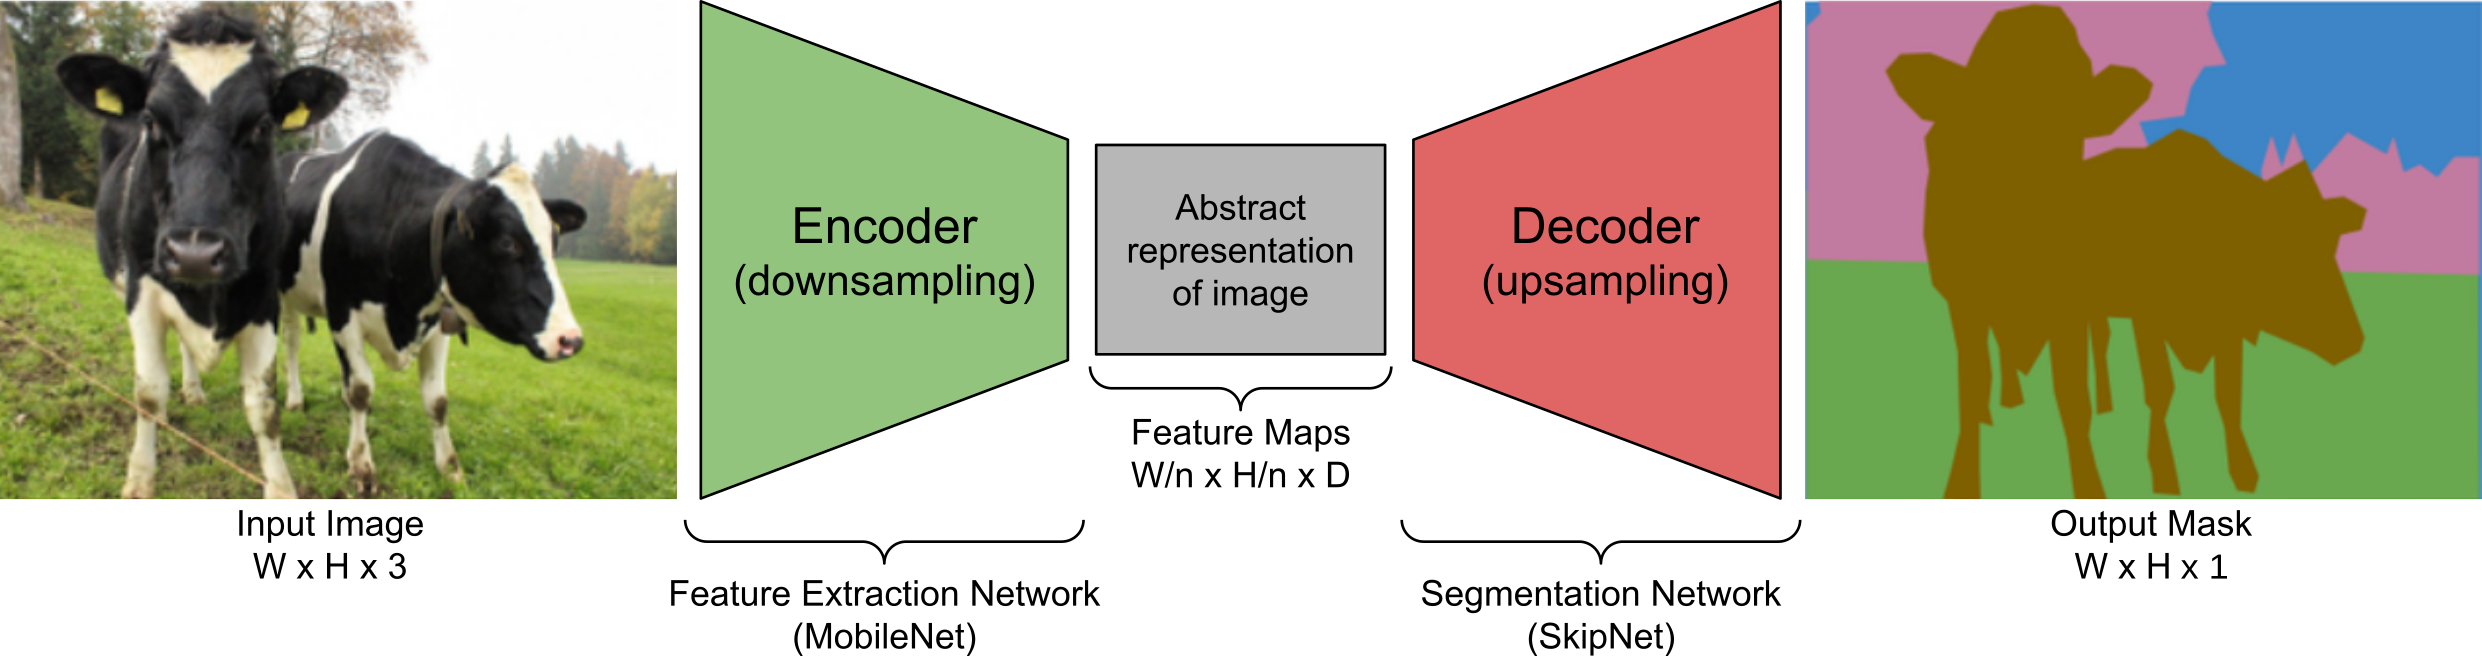
\includegraphics[width=12cm]{figures/Figure1.png}
    \caption{Esquema de la arquitectura de red FCN-MN propuesta en este trabajo, basada en la FCN propuesta por \citet{shelhamer2017fully}, reemplazando su encoder de extracción de features por las redes MobileNet \cite{howard2017mobilenets}, lo que produce features maps con un factor de downsampling $n$. Como decoder para la producción  del mapa de segmentación se utiliza la red SkipNet \cite{siam2018rtseg}, implementando las variantes 32s, 16s y 8s.}
    \label{fig:FCN-MN}
\end{figure}

Por otra parte, para refinar la calidad de la segmentación, se suelen utilizar conexiones que sobrepasan al menos una capa de la red, llamadas \emph{skip connections}. Éstas se utilizan para transferir información espacial local desde las capas internas del encoder directamente al decoder. En general, estas conexiones mejoran los resultados de segmentación, ya que mitigan la pérdida de información espacial permitiendo al decoder incorporar información de feature maps internos, aunque su impacto puede variar según la skip architecture que se proponga. En \citet{long2015fully} se proponen tres skip architectures: la 32s sin información de capas internas del encoder; la 16s que suma información espacial de capas profundas del encoder; y la 8s, que suma información espacial de capas profundas y menos profundas del encoder. Los detalles de estas arquitecturas quedan fuera del alcance de este trabajo, pero pueden consultarse en \citet{long2015fully} y \cite{shelhamer2017fully}. Dado que los resultados reportados en la literatura no son concluyentes respecto a que arquitectura es mejor \cite{long2015fully, shelhamer2017fully}, en este trabajo se consideran las tres alternativas.

A pesar de haber alcanzado excelentes resultados en la práctica,  estas arquitecturas conllevan una importante carga de recursos computacionales. Con esto en mente, en este trabajo se reemplazó el encoder VGG \cite{Simonyan2015VeryDC} propuesto originalmente por Long para las FCN, por la red MobileNet \cite{howard2017mobilenets}, una red que se destaca por tener tan solo $4.2$ millones de parámetros frente a los 138 millones de parámetros de VGG, permitiendo que el proceso de entrenamiento y testeo sea considerablemente más rápido, con requerimientos de memoria muy inferiores, pero manteniendo la performance. El uso de MobileNet como encoder en las fully convolutional netoworks de \citet{long2015fully} no es novedoso, sino que ha sido ya propuesto para la arquitectura 8s por \citet{siam2018rtseg} en su arquitectura SkipNet. Técnicamente, la propuesta de \citet{siam2018rtseg} es sumamente sencilla, por lo que nos atrevemos aquí a extenderla a las arquitecturas 16s y 32s propuestas originalmente por \citep{long2015fully}. Debido a estos cambios es que nos referimos a estas redes como \textbf{FCN-MN} de aquí a lo que resta del paper.


%------------------
\subsection{Sliding Windows detector}
\label{sec:sw}

En esta sección se describe el enfoque propuesto por \citet{perez2017image} para clasificación de imágenes de yema y una implementación del mismo para detección basada en sliding windows descrita en el trabajo original. A este enfoque de detección no referimos como SW de aquí a lo que resto del paper.

Este enfoque opera en tres pasos: (i) aplica el algoritmo de sliding windows sobre una imagen para extraer patches (sub-imágenes o regiones rectangulares); (ii) clasifica (todos los píxeles de) cada patch en yema o no-yema mediante el algoritmo presentado en \citet{perez2017image}; y (iii) produce la máscara de segmentación final mediante un esquema de votación. A continuación se dan los detalles de cada paso.

Las técnicas sliding windows comprenden una familia de algoritmos ampliamente utilizados en el pasado como parte de diversos enfoques para localización de objetos con bounding boxes \citep{divvala2009empirical, wang2009hog, chum2007exemplar, ferrari2007groups, dalal2005histograms, rowley1996human}. En estos algoritmos, cada imagen es escaneada densamente desde un extremo de la imagen (e.g. esquina superior izquierda) hasta el otro extremo (e.g. esquina inferior derecha) mediante una ventana deslizante rectangular en diferentes escalas y diferentes desplazamientos, extrayendo sub-imágenes o patches de la imagen original. En este trabajo, se definen 10 tamaños de ventana de igual alto y ancho, a saber 100, 200, 300, 400, 500, 600, 700, 800, 900 y 1000 píxeles, con un desplazamiento horizontal del $50\%$ el ancho de la ventana y un desplazamiento vertical del $50\%$ el alto de la ventana, lo que produce una superposición del $50\%$ entre parches contiguos. Estos valores se eligen sobre la base del análisis de robustez del clasificador que presenta \citet{perez2017image} para la geometría de la ventana. Este análisis muestra que el clasificador (explicado en la sección \ref{sec:swtrain}) es robusto para los patches que contienen al menos $60\%$ de los píxeles de una yema, y estos deben cubrir al menos el $20\%$ del patch. Si consideramos los casos extremos, i.e. el diámetro de yema más pequeño 100px y el más grande 1600px, tamaños de ventana de 100px y 1000px podrían contener al menos el 60% de los pixeles de una yema. Además utilizando un desplazamiento del 50%, se garantiza que al menos un patch contendrá más del 20% pixeles yema, 50px y 500px respectivamente. Los autores argumentan que un algoritmo de detección por sliding windows podría proponer fácilmente un esquema para elegir el tamaño y el desplazamiento de la ventana que garantice que en algún punto del escaneo la ventana satisface los requerimientos de robustez. Sin embargo no se dan detalles de cómo implementarlo, por lo que en este trabajo solo nos limitamos a reportar resultados para tamaños fijos de ventana y desplazamiento explicados. Dado que las yemas de la colección tienen un diámetro en píxeles variable (correspondientes a parches que varían de 100×100 a 1600×1600 píxeles aproximadamente) no todos los tamaños de ventana podrán satisfacer los requerimientos de robustez para todos los patches, pero los resultados todavía pueden ser útiles a los efectos de realizar la comparación con el enfoque FCN-MN.  

El segundo paso de este enfoque consiste en determinar si un patch es de clase yema o no-yema. El clasificador de \citet{perez2017image} toma los patches producidos por el sliding windows y para cada uno realiza las siguiente operaciones: (i) computa features visuales de bajo nivel mediante el algoritmo \emph{Scale Invariant Feature Transform} (SIFT) \cite{lowe2004distinctive}; (ii) construye un descriptor de alto nivel para cada patch empleando el algoritmo \emph{Bag of Features} (BoF) \cite{csurka2004visual} sobre los features SIFT del paso anterior; y (iii) determina la clase de cada patch usando el descriptor BoF sobre un clasificador construido mediante el algoritmo \emph{Support Vectors Machine} \cite{vapnik2013nature}. Los detalles del entrenamiento de este clasificador se posponen hasta la sección \ref{sec:swtrain} (Entrenamiento SW).

Finalmente, el tercer paso del enfoque consiste en construir la máscara binaria donde se encuentran etiquetados los píxeles que pertenecen a la clase yema y no-yema. Esta máscara es construida a través de un esquema de votación donde cada píxel suma un voto por cada patch que lo contiene clasificado como yema, el cual podría ser de un máximo de 4 para algunos píxeles debido a que el deslizamiento propuesto entre patches presenta solapamiento tanto horizontal como vertical. Luego, se establece un umbral de votos mínimos $\nu$ que puede tomar los valores del 1 al 4, de tal manera que los píxeles con una cantidad de votos igual o mayor a $\nu$ son clasificados como yema, caso contrario se clasifican como no-yema.



%---------------------------
\subsection{Entrenamiento de los modelos} 
\label{sec:train}

En esta sección se dan los detalles del proceso de entrenamiento para cada enfoque. Para poder contrastar ambos enfoques ambos se han diseñado para recibir el mismo tipo de entrada, i.e. una imagen de una escena vitícola, y para producir las mismas salidas, i.e. una máscara binaria del mismo tamaño que la imagen original cuyos píxeles positivos representan los pixeles del tipo yema, junto a las coordenadas (X,Y) de la localización de estas yemas. 
%
Esto permite entrenar ambos con la misma colección de imágenes, que se describe en el siguiente apartado, seguida de los detalles de entrenamiento específicos de cada modelo.

%------------------------
\subsubsection{Colección de imágenes}
\label{sec:collection}

La colección de imágenes utilizada en este estudio es la misma colección utilizada originalmente en \citet{perez2017image}, el cual se ha descargado de la URL http://dharma.frm.utn.edu.ar/vise/bc indicada por los autores. La colección completo está compuesta por 760 imágenes capturadas en condiciones natural de campo, en invierno. Sin embargo en este trabajo solo se tomaron las 698 imágenes que contienen exactamente una yema. Cada imagen está acompañada del ground truth, es decir una máscara con la segmentación manual de la yema. Estas imágenes y sus máscaras fueron empleadas durante el entrenamiento y evaluación de los modelos de detección. Para esto, la colección de imágenes se separó en dos subconjuntos disjuntos: el \emph{trainset} con el $80\%$ de las imágenes y el \emph{testset} con el restante $20\%$. Esto resultó en un trainset de 558 imágenes y un testset de 140 imágenes, ambos con sus respectivas máscaras ground truth. De esta manera, los dos enfoques propuestos utilizan exactamente las mismas 558 imágenes durante el entrenamiento, y las mismas 140 imágenes durante la evaluación.
%-----------------------------------


\subsubsection{Entrenamiento del enfoque FCN-MN.} 
\label{sec:fcntrain}

Para el entrenamiento de este enfoque se utilizaron las 558 imágenes reservadas para este propósito. Estas imágenes presentan diferentes resoluciones, sin embargo las tres FCN-MN propuestas requieren una entrada de tamaño fijo. Por esto, todas las imágenes (incluida sus máscaras) fueron escaladas a una resolución de $1024 \times 1024$ píxeles usando un método de interpolación bilinear \citep{han2013comparison}. Además, para las imágenes del trainset se realizó un scaling en los valores de intensidad RGB de los píxeles de [0,255] a [-1, 1].

Dado que la cantidad de imágenes en el trainset se considera escasa, para lograr un entrenamiento robusto se emplearon dos técnicas ampliamente utilizadas en la práctica: \emph{transfer learning} \cite{pan2009survey} y \emph{data augmentation} \cite{shorten2019survey}. El proceso de transfer learning se realizó de la siguiente manera: (i) se implementa la red MobileNet original propuesta en \citet{howard2017mobilenets}; (ii) se inicializa la red con los parámetros pre-entrenados sobre el dataset de benchmark ImageNet \cite{kornblith2019better}; (iii) se reemplaza la capa de clasificación multiclase de MobileNet por una capa de clasificación binaria; (iv) se entrena la red como un clasificador de patches yema y no-yema de forma análoga al entrenamiento de SVM, empleando el trainset de patches balanceado luego de escalar todas sus imágenes a $224 \times 224$ píxeles; y (v) se toman los parámetros obtenidos en el paso anterior para inicializar el encoder de nuestra FCN-MN, introducido en la sección \ref{sec:fcn}. El proceso de data augmentation se aplicó on the fly durante el entrenamiento, i.e. en la medida que el proceso requería nuevas imágenes. Por cada imagen del traiset se generaron 200 nuevas imágenes (111600 en total) aplicando simultáneamente las siguientes siete operaciones, donde sus valores se tomaron de forma aleatoria con probabilidad uniforme: \emph{rotación} de hasta $45\degree$; \emph{traslación horizontal} de hasta $40\%$; \emph{traslación vertical} de hasta $40\%$; \emph{shear} de hasta $10\%$; \emph{Zoom} de hasta $30\%$; \emph{flip horizontal}; y \emph{flip vertical}. 

%
Para el entrenamiento de las tres variantes de FCN-MN, la 8s, 16s, y 32s, se requiere especificar el \emph{método de optimización} y el valor de \emph{dropout}, dos parámetros típicamente definidos por el usuario. En este trabajo, los métodos de optimización que se tuvieron en cuenta fueron: \emph{Adam} con parámetros learning rate = $0.001$, $beta1 = 0.9$ y $beta2 = 0.999$; \emph{RMSProp} con parámetros learning rate = $0.001$ y $rho = 0.9$; y \emph{Stochastic Gradient Descent} con parámetros learning rate = $0.0001$ y $momentum = 0.9$. Para el caso de dropout se consideraron dos valores: $0.5$ y $0.001$. Estos valores fueron preseleccionados por experimentaciones preliminares que no se discuten aquí.
%
La mejor combinación de método de optimización y dropout se determinó en tiempo de entrenamiento sobre un conjunto de validación, utilizando el enfoque \emph{4-fold cross validation} por 60 epochs y batchsize igual a $4$, variando sobre los tres métodos de optimización y los dos valores de dropout. Los valores seleccionados fueron aquellos que maximizan el promedio de la Jaccard’s \emph{Intersection-over-Union} (IoU) \citep{jaccard1912distribution}, una medida de evaluación típica en problemas de segmentación (ver sección \ref{subsec:segmetrics}). Para cada combinación de valores de optimizer y dropout se reporta el promedio simple entre los $12$ IoU correspondientes a las $3$ variantes consideradas en cada uno de los $4$ folds. Observamos en la Tabla$\sim$\ref{tab:TablaX} que la combinación de parámetros con la que se alcanza mayor IoU promedio es RMSProp con dropout de $0.001$. 


\begin{table}[]
    \centering
    %\resizebox{0.5\textwidth}{!}
    \caption{Para cada combinación de valores de optimizer y dropout se reporta el promedio simple entre los $12$ IoU correspondientes a las $3$ variantes consideradas en cada uno de los $4$ folds.}
    \label{tab:TablaX}
\end{table}


Finalmente se procedió a entrenar las 3 variantes con RMSProp como método de optimización y un valor de dropout de $0.001$ sobre el conjunto de entrenamiento completo por 200 epochs y batchsize igual a 4.

\subsubsection{Entrenamiento enfoque SW} 
\label{sec:swtrain}


La etapa de entrenamiento para este enfoque se realiza de la misma manera que para el workflow original propuesto en \citet{perez2017image}. Esto implica entrenar un clasificador binario para que aprenda el concepto de yema versus no-yema a partir de una colección de patches rectangulares que contienen o no una yema. Durante el entrenamiento, los patches yema deben ser regiones que circunscriben perfectamente la yema mientras que los  patches no-yema deben ser regiones que no contienen ni un solo píxel de yema (ver$\sim$\ref{fig:Figure2}). Por lo tanto, para construir la colección de parches, se procesaron las $558$ imágenes y sus máscaras siguiendo el mismo protocolo que en \citet{perez2017image}, obteniendo un total de $558$ patches que circunscriben a cada yema (existe una por imagen) y más de $25000$ patches no-yema (el área no-yema es mucho mayor al área que ocupa una yema en la imagen). El tamaño de estos patches es variable, con resoluciones entre $0.1$ y $2.6$ megapíxeles aproximadamente (patches de $100 \times 100$ a $1600 \times 1600$ píxeles).



\begin{figure}
    \centering
    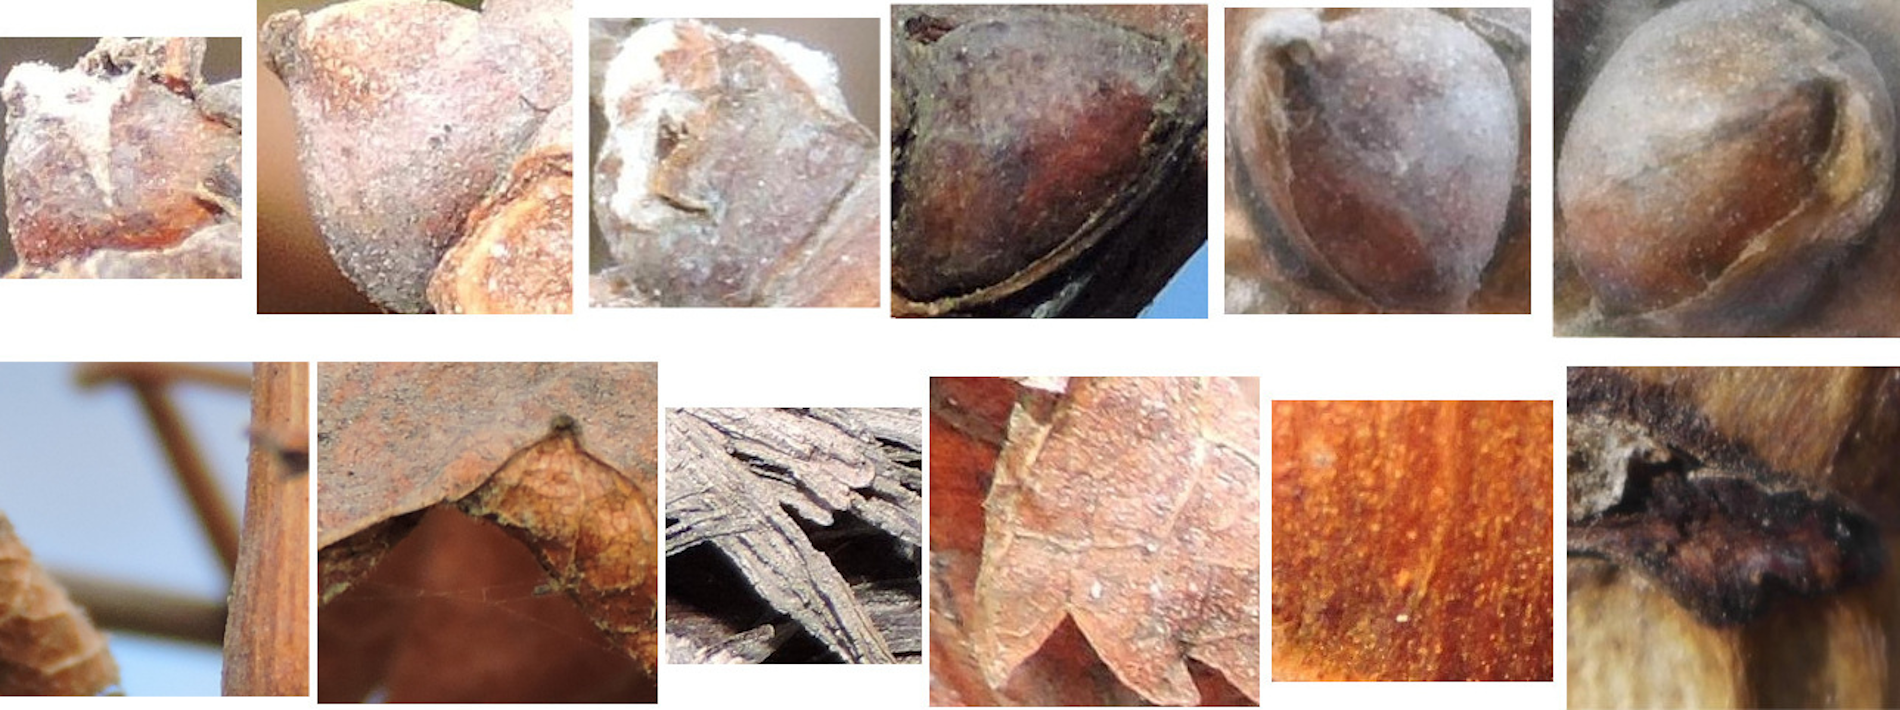
\includegraphics[width=12cm]{figures/Figure2.png}
    \caption{Collection of patches used in this work. The first and second rows correspond to bud patches and non-bud patches, respectively. Image extracted from \citet{perez2017image}.}
    \label{fig:Figure2}
\end{figure}

A partir de esta colección de parches, se creó un trainset de parches balanceado, i.e. con 558 patches de cada clase, donde los patches no-yema fueron tomados al azar entre miles de patches. El entrenamiento se realizó tal como se detalla en el pipeline propuesto en \citet{perez2017image}: (i) se extrajeron descriptores SIFT todos los patches del trainset; (ii) se aplicó BoF con tamaño de vocabulario igual a 25, dado que fue el modelo con mejores resultados según los autores; y (iii) se entrenó el clasificador SVM sobre los descriptores BoF de cada patch, empleando un kernel \emph{Radial Basis Function}, donde el valor de los parámetros $\gamma$ y $C$ se estableció mediante un 5-fold cross-validation sobre los mismos rangos de valores, i.e. $\gamma = \{2^{-14}, 2^{-13}, \ldots, 2^{-7}\}$ y $C = \{2^{5}, 2^{6},\ldots , 2^{14}\}$.

%%%%%%%%%%%%%%%%%%%%%%%%%%%%%%%%%%%%%

\section{Experimental results} \label{sec:results}

In this section we present a systematic evaluation of the quality our proposed procedure FCN-MN for bud detections quality, which, according to the discussion in the introduction, can be decomposed on the three aspects that impact on the relevant bud related variables listed in Table$\sim$\ref{tab:TableX}: \emph{segmentation}, \emph{correspondence identification}, and \emph{localization}. 

%
For that, we start in the following subsection by presenting metrics that quantify the quality for these aspects, followed by the results subsection$\sim$\ref{sec:results} that presents details on the metric values obtained for different experiments over the test set of images. 


\subsection{Performance metrics} \label{sec:metrics}

% The main challenge for quantifying the errors for the three aspects of detection requires the understanding that the detection produced by both FCN-MN and SW algorithms consists of associating each \emph{connected component} of the output binary masks with one detected bud.


% Then, we refine the evaluation by reporting  the quality of the segmentation for those connected components that correctly detected a bud. We start in the following section by defining the metrics used to validate both detection and segmentation, and then proceed to compare the results of applying those metrics to the masks produced by our FCN-MN approach against those of the SW approach of cite{perez2017image} (c.f. Section$\sim$\ref{sec:sw}), over all 140 images of the test collection.


\subsubsection{Correspondence identification metrics } \label{subsec:detectmetrics}

Correspondence identification of buds, in both FCN-MN and SW, is the result of two steps: (i)  the thresholding of the algorithm’s output mask into a \emph{binary mask}, keeping all pixels of $\nu$ the probabilistic mask output by FCN-MN with values higher than $\tau$ and keeping all pixels belong to at least $\nu$ patches rendered positive by SW, and (ii) the association of each \emph{connected component} of the binary mask to exactly one (detected) bud. 

%
An incorrect correspondence identification is thus the result of incorrect matching of detected components with actual buds in the image. This matching can get very complicated when there is an unknown number of true buds in the scene as can be seen by the large amount of possible detection metrics defined in \cite{oguz2017dice}. To simplify the analysis our image collection contains a single bud per image, avoiding the need of all metrics that report the confusing situation of a component overlapping more than one true bud. This results in the following simplified list of possible metrics:

\begin{itemize}
\item \textbf{Correct Detection} ($CD$) is the best case, and counts all images in the test collection for which the detected binary mask presents a single connected component, and this connected component overlaps with the true bud of the image. This would correspond with a \emph{true positive} situation.
\item \textbf{Split} ($S$) occurs when there is more than one detection per bud, which happens  when the mask contains multiple connected components, all of which overlaps the true bud. This metric counts the total number of images of the test collection whose detection is splitted.
\item \textbf{False Alarm} ($FA$), is equivalent to a \emph{false positive} situation, and corresponds to connected components not overlapping with the true bud. This measure counts the total number of such components over all images in the test collection.
\item \textbf{Detection Failure} ($DF$), is equivalent to a \emph{false negative} situation,when the detection mask presents no connected components. It counts one each image satisfying this condition.
\end{itemize}

All four of these cases are mutually exclusive, that is, no image can satisfy any two (or more) of these definitions simultaneously. To quantify the correspondence identification quality one could simply report these quantities counted over the test set, with the best case consisting in a $CD$ value equal to the cardinality of this set. However, determining the overall correspondence identification quality from the analysis of $4$ quantities can get rather complicated. 
%
One alternative is reporting the well-known precision and recall, denoted $P_D$ and $R_D$ and referred to as  \emph{detection-precision} and \emph{detection-recall} to distinguish them from the segmentation precision and recall defined later below. For that, we have to address first the fact that  we have two differing true positive counts: $CD$ and $S$. We solve this by first counting as true positives not only the $CD$ type of images, but the $S$ ones, i.e., we count as one true positive any image with either a correct detection or a split case, resulting in:

\begin{equation}
    P_D = \frac{true\ positives}{true\ positives+false\ positives} \\
= \frac{CD+S}{CD+S+FA}
    \label{eq:detection-precision}
\end{equation}

\begin{equation}
    R_D = \frac{true\ positives}{true\ positives+false\ negatives} \\
= \frac{CD+S}{CD+S+DF},
    \label{eq:detection-recall}
\end{equation}
and then account for the split type of errors by explitictely reporting $S$. 

Given these quantities we also report the \emph{F1-measure} computed as their harmonic average:
\[
    F1 = 2 \times \frac{precision \times recall}{precision + recall}.
\] 

%%%%%%%

 \subsubsection{Segmentation metrics} \label{subsec:segmetrics}

Correspondence identification metric, although informative, relies on  the overlap between the detected and true buds, regardless of how minimal the overlap. This could miss several possible pixelwise detection errors, resulting in rather coarse comparisons between competing detection algorithms. For instance, a correct detection could present a very small overlap with the true bud, with many or even a majority of the true bud’s pixels missing (i.e., several \emph{false negatives} pixels), or could be erroneously reporting several pixels as bud pixels (i.e., several \emph{false positives} pixels). Clearly, the best case scenario would be a case of correct detection with no false negative or positive pixels, that visually would correspond to a perfect overlap of the detected connected component and the true bud. 
%
Similarly, a pixel wise comparison of the masks could help assess the quality of the splits. The best split, for instance, would be one completely enclosed within the true mask, i.e., with none of its connected components presenting false positive pixels; while covering as much of the true bud mask as possible, i.e., presenting just enough false negatives to disconnect its components. 
%
Finally, a false alarm case, clearly presenting only false positive pixels, could be further assessed by the number of (false positive) pixels in its components. 

The community has proposed several metrics to quantify segmentation errors. The most obvious ones are those that 
report the \emph{fraction} of the whole image corresponding to \emph{true positive} pixels, denoted $TPF$; \emph{false positive} pixels,  denoted $FPF$;  and \emph{false negative} pixels, denoted $FNF$. 
%
As for the correspondence identification metrics, one can simplify the analysis by considering the  pixelwise precision and recall, denoted $P_S$ and $R_S$ and referred to as \emph{segmentation precision}  and \emph{segmentation recall}, defined formally as: 

\begin{eqnarray*} 
    P_S &=& TPF / (TPF + FPF) \\
    R_S &=& TPF / (TPF + FNF),
\end{eqnarray*}
% Another combination of these quantities, useful to assess the relative size of the false positives, is the \emph{false-positive-rate}, computed as $FPF/(FPF + TNF)$, or simply $FPF / NF$, where the latter is the fraction of negatives, that is, all except the true bud pixels. 
% But even these two quantities can be simplified into a single quantity in two different ways. accompanied by their weighted harmonic mean, the well-known \emph{F-measure}, 

\begin{equation} 
   2 \times precision \times recall / (precision + recall),
\end{equation}

proposed independently by \citet{dice1945measures}, thus usually referred to as the \emph{Dice measure}. A common alternative to the Dice measure is the  Jaccard’s \emph{intersection-over-union} \citep{jaccard1912distribution}, 
equivalent to $TPF / (TPF+FPF+FNF)$. 

With these metrics, one could quantify the refinements discussed in the first paragraph above, by simply applying them, no to the whole mask, but to the individual correspondence identification cases. For instance, reporting the mean Dice measured over all correctly detected components; or, to refine the assessment of how bad is a split, one could report the mean Dice measure to all components of some split, or the mean Dice measure over all split components of all split images. 

The case of false alarms is rather monotonous and not very informative, with zero precision and recall for all such components. Indeed, a pixelwise assessment of the gravity of a false alarm requires a quantification of the number of false positive pixels. One could simply consider the $FPF$, the fraction of all the image pixels that are false positives. Instead, we considered a normalization against the size of the bud to be more informative, resulting in the \emph{normalized area}, denoted $NA$ and defined formally as  \emph{the total area of the component corresponding to its total number of pixels, normalized by the area of the true bud}. 

%One could report the mean \emph{false-positive-rate} , computed as $FPF/(FPF + TNF)$, or simply $FPF / NF$, over all images, to assess the gravity of the false alarm components produced by some algorithm.  This qua

% Segmentation results for correct detection and splits allowed us to further assess the quality of the detections. However, as shown by the detection precision and recall results above, there is no lack of false detections, the false positive components we called false alarms. For instance, in their best versions, $2.3\%$ of all components produced by the FCN-MN with threshold $0.8$ and architecture 16s are false alarms, increasing to $33\%$ for the case of SW with voting threshold 1 and windows size 1000px.  These percentages, however, do not tell us how bad these false alarms are. Whether they are large or small, or whether they are located nearby the true bud (appearing more as splits than false alarms) or they are further away. 

 \subsubsection{Localization metrics} \label{subsec:locmetrics}

As a localization metric we propose the \emph{normalized distance}, denoted $ND$, defined formally as \emph{the distance between the center of mass of the component, to the center of mass of the true bud, divided by the diameter of the true bud (defined as the maximum distance between any two border points of the true bud)}.


%%%%%%%%%%%%%%%%%%%%%%%%%%%%%%%%%%%%%%%%%%%%%%%%%%

\subsection{Results}   \label{sec:resultados}

We proceed now to assess the validity of our main hypothesis, namely, that FCN-MN is a better detector than its SW counterpart over each of the metrics defined in the previous section. 

For a thorough comparison we considered several cases for each algorithm, training $27$ FCN-MN detectors and $40$ SW detectors over the training set of $558$ images, one for each combination of their respective hyper-parameters. For FCN-MN these hyper-parameters are the three architectures 8s, 16s, and 32s, and the $9$ values $\{0.1, 0.2, \ldots, 0.9\}$ for the binarization threshold $\tau$; whereas for SW these hyper-parameters are the $10$ patch sizes $\{100, 200, \ldots, 1000\}$  and the $4$ values $\{1, 2, 3, 4\}$  of the voting threshold $\nu$.


Table$\sim$\ref{tab:TablaXX} shows the results for the best detectors of each algorithm, reporting all performance metrics of the three aspects of detection: correspondence identification, segmentation and localization. The first column shows the label of the selected detectors, with the subscript indicating the architecture and patch size for the case of FCN-MN and SW, respectively, while the superscript indicating the thresholds $\tau$ and $\nu$, respectively.

%COLUMNS - METRICS
The table includes all metrics defined in Section$\sim$\ref{sec:metrics} required for a thorough comparison of FCN-MN against SW. First, we include four correspondence identification metrics: detection precision $P_D$, detection recall $R_D$, the F1-measure  $F1$, and $S$ (the total count of split components). 
%
For a thorough analysis of the segmentations we discriminated the segmentation metrics for the correctly detected, splitted and false alarms. For the detections, i.e., correctly detected and splits, we report segmentation precision,  segmentation recall, and the Dice measure denoted in the table by $P_S^{CD}$, $R_S^{CD}$ and $Dice^{CD}$ for the correctly detected, and $P_S^S$, $R_S^S$ and $Dice^S$ for the splits.  Each of the three correctly detected cells report the mean value of the measure computed for each correctly detected test image, i.e., each image with only one component overlapping the true bud, including the corresponding standard deviation  in parenthesis. For the split group, the mean and standard deviation are computed over the measures computed only for the split images, i.e., over the images containing at least two components overlapping the true bud. Here, the segmentation metrics are computed over the union of all split components. 
%
For the false alarms we reported the mean \emph{normalized area}($NA$), in this case computed individually for each false alarm component, reporting at each cell its mean over all false alarm components of all test images. 

Finally, for localization the table reports the \emph{normalized distance}($ND$) only for false alarms, considering that correctly detected and splits, as they overlap the true bud, should be close enough to render it unnecessary further analysis. Instead, a false alarm can be arbitrarily far from the true bud.  We thus report in the column $ND$ the mean normalized distance of each false alarm connected component that appears in any test image.

% ROWS - MODELS INCLUDED
The table is a summary, as it includes only a subset of all $27$ FCN-MN cases, and a subset of all $40$ SW cases. A detector was considered for inclusion in the table if, when compared to its counterparts of the same algorithm, it resulted in the higher value for at least one of the metrics. The corresponding cell was marked in bold in the table. For instance, the detectors FCN-MN$_{16s}^{0.8}$ is included because its detection precision $P_D$ of $97.7$ is the largest among the detection precision of all $27$ FCN-MN detectors. Similarly, the detectors SW$_{1000}^1$ has been included because its precision $P_D = 67.0$is the largest among all $40$ SW detectors. 


% RESULTS
The table shows a clear improvement of FCN-MN over SW. For all metrics it is the case that the best  FCN-MN detector (bolded) improves (or ties) over the best SW detector (bolded); represented in the table by underlying the one with better metric; with the exception of the two segmentation recalls (for correctly detected and splits) for which the SW case has a better (larger) mean, $98.8$ versus $99.9$ for correctly detected, and $74.7$ versus $78.6$ for the split case; and the total split count $S$, with the best case for FCN-MN being $1$ and $0$ for the best SW case. These improvements are not statistically significant, however, due to the large standard deviations of the FCN-MN cases, of $3.4$ and $8.1$, for the correctly detected and split cases, respectively,  resulting in (statistically) overlapping values. 
%
In some cases the improvements of FCN-MN over SW are overwhelming. For instance, for the detection-precision, the correctly detected segmentation-precision, and the split segmentation-precision, the FCN-MN over SW improvements are $97.7$ versus $67.0$, $98.1$ versus $46.5$ and $99.9$ versus $67.5$, respectively.  Also, for $NA$ and $ND$ the  FCN-MN versus SW improvements are $0.04$ versus $0.22$, and $1.1$ versus $6.0$, respectively.





\begin{table}[]
    \scriptsize
    %\tiny
    \centering        
    \begin{adjustbox}{angle=90}
        \resizebox{.90\textheight}{!}{%
           \begin{tabular}{lcccccccccccc}
                \hline
                \multicolumn{1}{|l|}{\textbf{Detector}} & \multicolumn{1}{c|}{\textbf{$P_D$}} & \multicolumn{1}{c|}{\textbf{$R_D$}} & \multicolumn{1}{c|}{\textbf{$F1$}} & \multicolumn{1}{c|}{\textbf{$S$}} & \multicolumn{1}{c|}{\textbf{$P_S^{CD}$}} & \multicolumn{1}{c|}{\textbf{$R_S^{CD}$}} & \multicolumn{1}{c|}{\textbf{$Dice^{CD}$}} & \multicolumn{1}{c|}{\textbf{$P_S^S$}} & \multicolumn{1}{c|}{\textbf{$R_S^S$}} & \multicolumn{1}{c|}{\textbf{$Dice^S$}} & \multicolumn{1}{c|}{\textbf{$NA$}} & \multicolumn{1}{c|}{\textbf{$ND$}} \\ \hline
                FCN-MN$_{8s}^{0.5}$ & 75.4 & 98.6 & 85.4 & 2 & 91.0 (11.3) & 90.2 (11.7) & {\ul \textbf{89.6 (10.3)}} & 96.6 (2.2) & 73.1 (17.6) & {\ul \textbf{82.1 (10.2)}} & 0.26 (0.69) & 3.72 (4.64) \\
                FCN-MN$_{8s}^{0.9}$ & 90.1 & 97.1 & 93.5 & 8 & {\ul \textbf{98.1 (6.0)}} & 68.3 (21.1) & 77.9 (19.6) & 98.7 (3.0) & 57.4 (18.4) & 70.8 (13.6) & 0.24 (0.5) & 3.8 (5.66) \\
                FCN-MN$_{16s}^{0.1}$ & 71.3 & {\ul \textbf{100}} & 83.2 & 6 & 75.7 (13.1) & 95.4 (14.7) & 83.1 (13.5) & 83.1 (8.9) & 54.1 (21.9) & 61.9 (17.5) & 0.12 (0.44) & 5.27 (6.53) \\
                FCN-MN$_{16s}^{0.4}$ & 87.0 & 96.4 & 91.5 & \textbf{1} & 87.7 (12.1) & 89.8 (18.2) & 87.0 (15.6) & 96.7 (0.0) & 37.0 (0.0) & 53.5 (0.0) & {\ul \textbf{0.04 (0.09)}} & 3.8 (5.08) \\
                FCN-MN$_{16s}^{0.6}$ & 95.6 & 93.6 & 94.6 & 3 & 92.2 (8.7) & 88.2 (13.3) & 89.1 (10.7) & 99.4 (0.6) & 16.2 (10.6) & 26.6 (16.8) & 0.08 (0.11) & {\ul \textbf{1.1 (0.65)}} \\
                FCN-MN$_{16s}^{0.8}$ & {\ul \textbf{97.7}} & 92.1 & {\ul \textbf{94.9}} & 4 & 95.8 (7.0) & 81.6 (14.6) & 87.0 (10.7) & 99.7 (0.3) & 34.2 (32.6) & 43.9 (33.1) & 0.1 (0.12) & 1.28 (0.95) \\
                FCN-MN$_{16s}^{0.9}$ & {\ul \textbf{97.7}} & 91.4 & 94.5 & 4 & 97.6 (5.6) & 74.5 (16.5) & 83.1 (12.8) & {\ul \textbf{99.9 (0.1)}} & 31.8 (27.9) & 41.6 (34.0) & 0.07 (0.11) & 1.33 (0.9) \\
                FCN-MN$_{32s}^{0.1}$ & 35.4 & {\ul \textbf{100}} & 52.2 & 8 & 67.4 (14.0) & \textbf{98.8 (3.4)} & 79.1 (11.0) & 86.0 (9.4) & 73.4 (19.6) & 77.1 (10.4) & 0.14 (0.66) & 4.62 (5.59) \\
                FCN-MN$_{32s}^{0.2}$ & 50.9 & {\ul \textbf{100}} & 67.5 & 10 & 73.9 (13.6) & 98.1 (3.8) & 83.5 (10.1) & 92.2 (5.4) & 53.4 (25.8) & 63.6 (19.3) & 0.17 (0.55) & 4.33 (6.17) \\
                FCN-MN$_{32s}^{0.3}$ & 49.8 & {\ul \textbf{100}} & 66.5 & 10 & 79.1 (13.2) & 95.5 (10.5) & 85.2 (11.8) & 88.5 (9.7) & 61.0 (35.1) & 65.8 (28.2) & 0.1 (0.39) & 3.68 (5.62) \\
                FCN-MN$_{32s}^{0.6}$ & 68.5 & 99.3 & 81.1 & 16 & 89.0 (11.5) & 89.1 (11.3) & 88.1 (9.6) & 92.4 (7.7) & \textbf{74.7 (28.1)} & 78.1 (24.0) & 0.11 (0.3) & 2.95 (4.36) \\
                SW$_{100}^{1}$ & 9.4 & {\ul \textbf{100}} & \textbf{17.2} & 28 & 24.6 (17.7) & 86.7 (19.5) & 33.6 (15.1) & 57.9 (28.2) & 24.8 (16.8) & 27.9 (13.8) & 1.08 (3.2) & 7.68 (6.02) \\
                SW$_{100}^{3}$ & 14.6 & 93.1 & 25.3 & 40 & 42.4 (26.4) & 56.8 (29.9) & \textbf{39.9 (19.7)} & 55.5 (32.2) & 24.8 (18.1) & 26.0 (15.6) & 0.31 (0.96) & 6.45 (6.19) \\
                SW$_{100}^{4}$ & 19.5 & 87.4 & 31.9 & 49 & \textbf{46.5 (29.3)} & 39.2 (28.9) & 33.9 (21.1) & 49.0 (29.0) & 20.1 (13.7) & 24.1 (14.0) & \textbf{0.22 (0.57)} & \textbf{6.0 (6.56)} \\
                SW$_{200}^{1}$ & 20.0 & {\ul \textbf{100}} & 33.3 & 12 & 16.6 (12.5) & 94.9 (13.5) & 25.9 (14.2) & 49.3 (26.4) & 40.2 (17.4) & 36.8 (11.9) & 5.13 (19.3) & 7.56 (5.35) \\
                SW$_{200}^{3}$ & 26.0 & 98.6 & 41.1 & 19 & 29.9 (17.0) & 74.7 (27.3) & 38.5 (17.0) & \textbf{67.5 (32.7)} & 16.5 (8.9) & 24.2 (11.9) & 1.69 (3.15) & 8.94 (6.22) \\
                SW$_{300}^{1}$ & 26.9 & {\ul \textbf{100}} & 42.4 & 2 & 13.7 (13.6) & 97.0 (9.6) & 21.6 (15.5) & 55.0 (11.8) & 48.1 (1.1) & \textbf{50.8 (4.5)} & 7.79 (20.5) & 6.83 (4.44) \\
                SW$_{400}^{1}$ & 32.7 & {\ul \textbf{100}} & 49.3 & 2 & 10.5 (11.7) & 98.7 (9.3) & 17.2 (15.3) & 42.6 (10.1) & 61.9 (11.6) & 50.4 (10.9) & 11.59 (24.05) & 7.12 (4.15) \\
                SW$_{400}^{2}$ & 34.6 & {\ul \textbf{100}} & 51.4 & 4 & 15.6 (15.1) & 94.5 (13.3) & 23.8 (15.6) & 48.7 (27.6) & 36.0 (4.6) & 38.6 (13.1) & 9.54 (26.13) & 7.88 (4.89) \\
                SW$_{500}^{1}$ & 40.2 & {\ul \textbf{100}} & 57.3 & 1 & 8.40 (9.7) & {\ul \textbf{99.9 (4.9)}} & 14.2 (13.8) & 17.9 (0.0) & {\ul \textbf{78.6 (0.0)}} & 29.2 (0.0) & 17.39 (30.07) & 7.22 (4.04) \\
                SW$_{500}^{2}$ & 38.6 & {\ul \textbf{100}} & 55.7 & 1 & 13.5 (14.0) & 95.2 (14.5) & 21.0 (16.0) & 35.2 (0.0) & 45.9 (0.0) & 39.8 (0.0) & 17.19 (39.07) & 7.56 (4.42) \\
                SW$_{600}^{1}$ & 43.5 & {\ul \textbf{100}} & 60.6 & {\ul \textbf{0}} & 6.9 (7.8) & 98.5 (10.7) & 12.0 (12.0) & nan (nan) & nan (nan) & nan (nan) & 25.48 (48.45) & 7.72 (4.3) \\
                SW$_{600}^{2}$ & 41.7 & {\ul \textbf{100}} & 58.8 & 1 & 10.4 (10.6) & 93.7 (18.9) & 17.2 (14.4) & 19.7 (0.0) & 27.2 (0.0) & 22.9 (0.0) & 20.41 (38.32) & 7.92 (4.38) \\
                SW$_{700}^{1}$ & 50.6 & {\ul \textbf{100}} & 67.2 & {\ul \textbf{0}} & 5.6 (6.5) & 98.6 (12.0) & 9.9 (10.3) & nan (nan) & nan (nan) & nan (nan) & 31.95 (64.36) & 7.75 (4.45) \\
                SW$_{800}^{1}$ & 56.7 & {\ul \textbf{100}} & 72.4 & {\ul \textbf{0}} & 5.1 (6.6) & 97.7 (11.0) & 9.0 (10.4) & nan (nan) & nan (nan) & nan (nan) & 44.53 (71.52) & 7.7 (4.06) \\
                SW$_{800}^{2}$ & 49.6 & 99.2 & 66.1 & {\ul \textbf{0}} & 8.3 (9.4) & 95.0 (15.9) & 13.9 (13.2) & nan (nan) & nan (nan) & nan (nan) & 30.52 (46.45) & 7.82 (4.1) \\
                SW$_{900}^{1}$ & 64.3 & {\ul \textbf{100}} & 78.3 & {\ul \textbf{0}} & 4.2 (5.7) & 94.7 (19.0) & 7.5 (9.2) & nan (nan) & nan (nan) & nan (nan) & 48.16 (80.31) & 7.9 (4.35) \\
                SW$_{900}^{3}$ & 42.2 & 92.4 & 58.0 & {\ul \textbf{0}} & 15.0 (14.8) & 81.5 (28.9) & 22.7 (16.8) & nan (nan) & nan (nan) & nan (nan) & 17.97 (29.56) & 7.65 (4.67) \\
                SW$_{1000}^{1}$ & \textbf{67.0} & {\ul \textbf{100}} & \textbf{80.2} & {\ul \textbf{0}} & 3.7 (4.7) & 95.3 (18.3) & 6.8 (7.9) & nan (nan) & nan (nan) & nan (nan) & 57.83 (84.87) & 7.91 (4.3) \\
                SW$_{1000}^{2}$ & 56.7 & 98.3 & 71.9 & {\ul \textbf{0}} & 6.3 (6.9) & 93.8 (19.1) & 11.1 (10.9) & nan (nan) & nan (nan) & nan (nan) & 47.26 (68.92) & 7.98 (4.44) \\ \hline
            \end{tabular}     
        }
    \end{adjustbox}
    \caption{Correspondence identification, segmentation and localization metrics for the best FCN-MN and SW detection models.   Each column shows two bolded cells, corresponding to the cell with better metric among all FCN-MN rows, and the cell with better metric among the SW rows. The larger of the two has been underlined, representing the best among all combined models, i.e., the best of the column.  Columns $P_D$, $R_D$, $F1$, and $S$ show results for the \emph{Correspondence identification metrics} detection precision, detection recall, the F1-measure and the number of images with splits, respectively: Columns $P_S^{CD}$, $R_S^{CD}$ and $Dice^{CD}$ (resp. $P_S^S$, $R_S^S$ and $Dice^S$) correspond to the \emph{segmentation metrics} mean segmentation precision, mean segmentation recall, and the mean Dice measure over all correctly detected components (resp. split components); and Columns $NA$ and $ND$ show the mean $NA$ and mean $ND$ over all false alarm components.}
        \label{tab:TablaXX}
    \end{table}

\subsubsection{Detailed analysis of correspondence identification metrics} 
\label{sub:compFCNSW}

% We start by reporting the comparison of detection-precision and detection-recall, to then analyze how many of the true positives involved are indeed splits.  

Graphically one could expect a better combined analysis of the detection-precision and detection-recall than one could obtain by comparing the F1-measure. This is shown as a scatter plot in Figure$\sim$ref{fig:detection-scatter-plot}, a graphical representation of a non-summarized version of the second and third columns of Table$\sim$\ref{tab:TablaXX}. Each dot  in the plot is located according to the detection-precision and detection-recall, and the colored black or white whether it corresponds to an FCN-MN or an SW detection model.
%
The graph reinforces the clear and undisputed improvements of FCN-MN over SW already detected in the table, with similar detection-recalls but larger detection-precisions over the majority of scenarios. 




 \begin{figure}
    \centering
    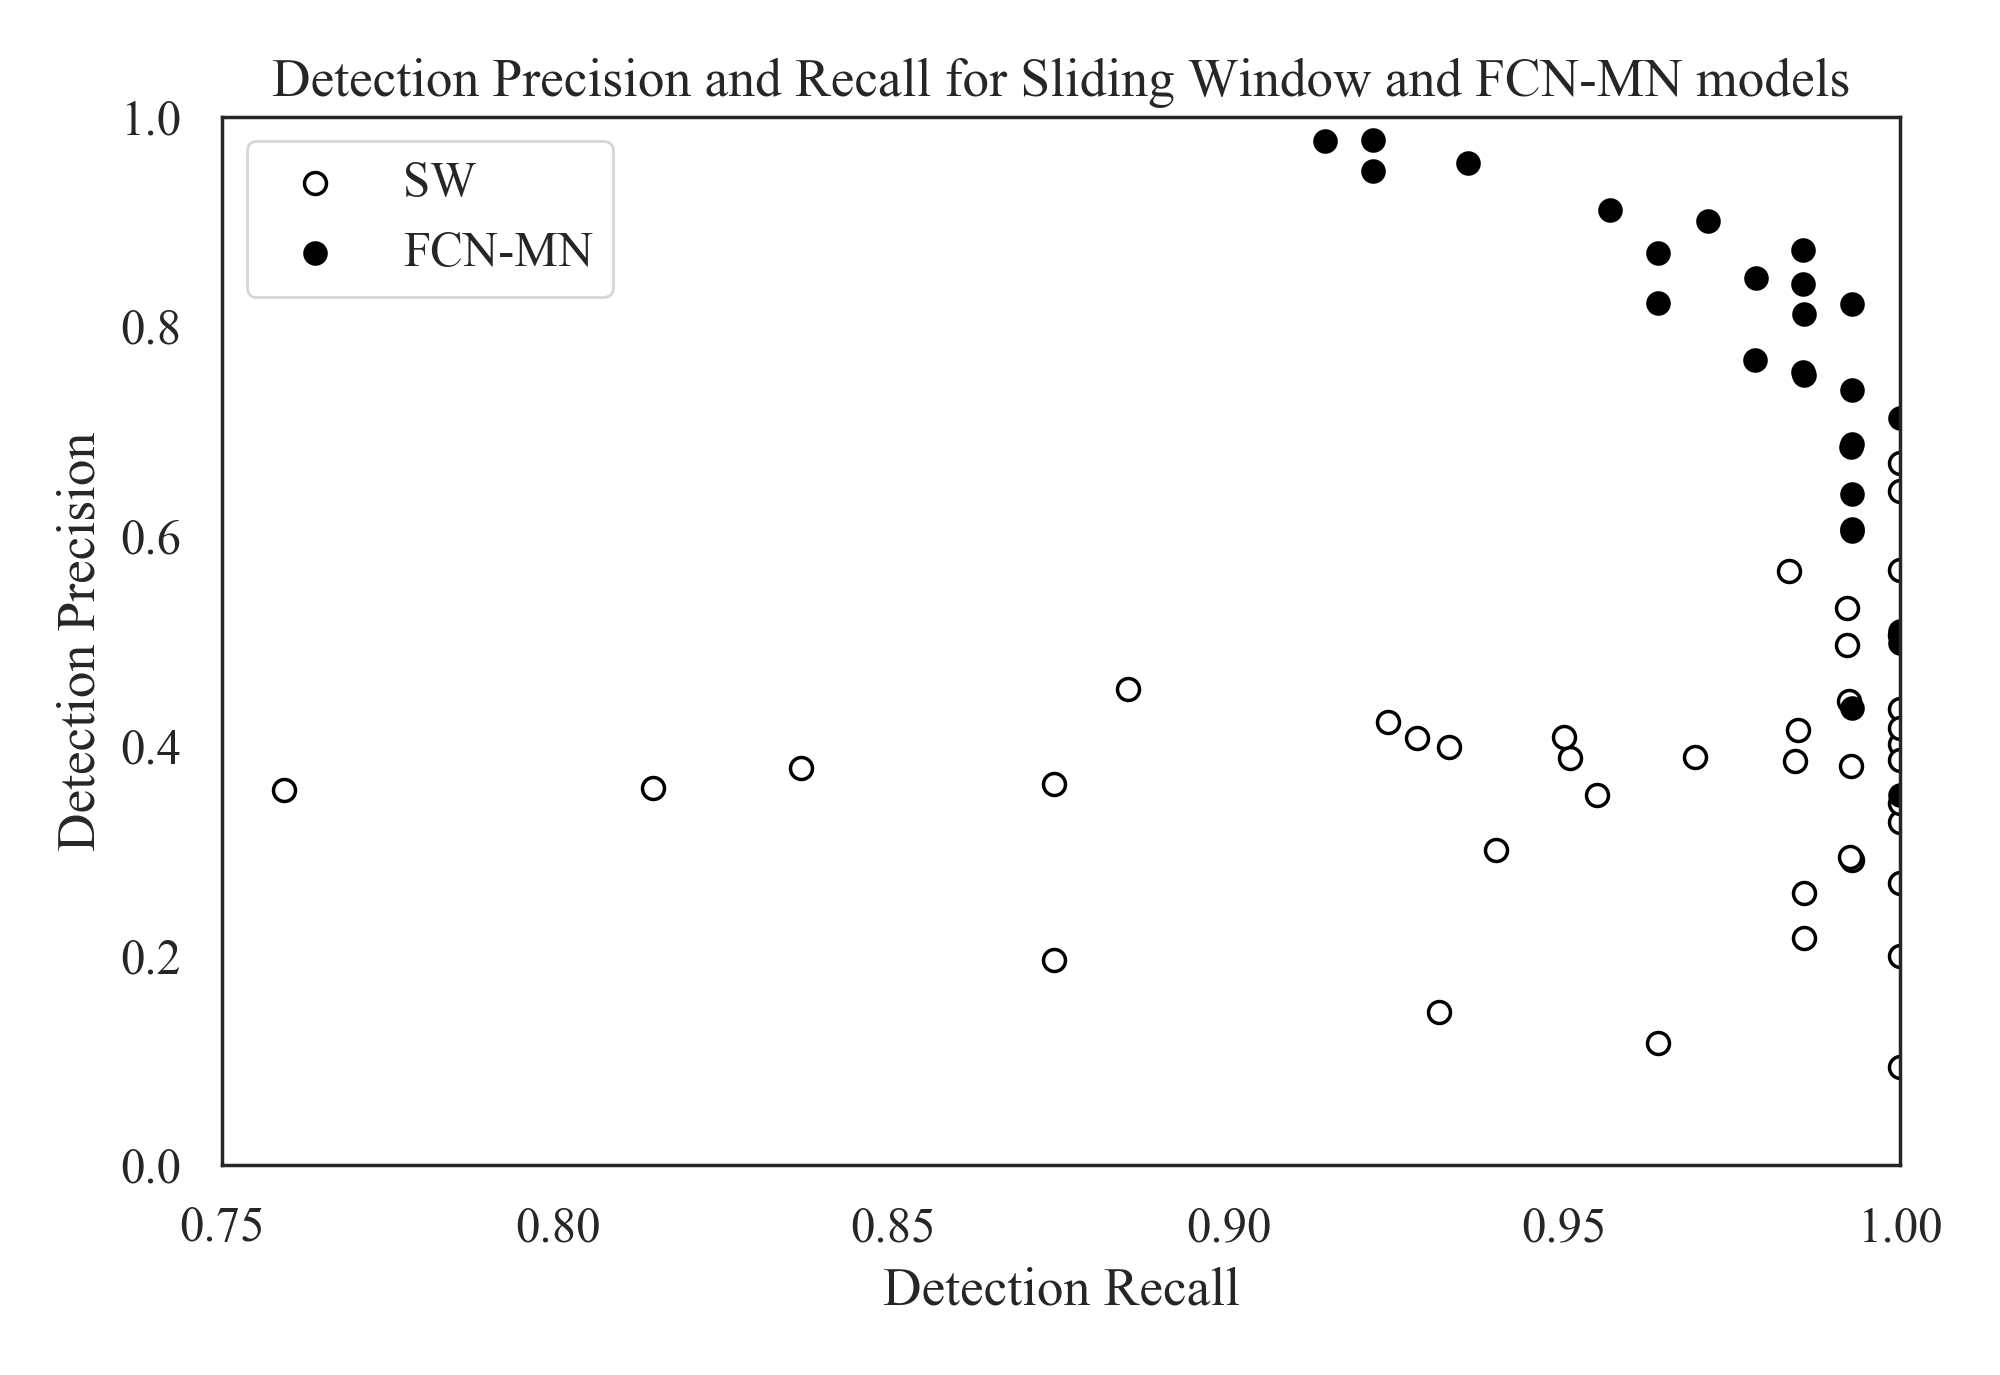
\includegraphics[width=\textwidth]{figures/111_precision_recall_detection.png}
    \caption{Precision-Recall scatterplots of the second and third columns of Table$\sim$\ref{tab:TablaXX} discriminating the results for FCN-MN and SW with black and white dots, respectively. Each dot then  represents the detection-precision and detection-recall computed over all images of the tests, for some particular  configurations of hyperparameters. For FCN-MN, these would be the architecture, with values 8s, 16s and 32s, and threshold $\tau = \{0.1, 0.2, \ldots, 0.9\}$,  for a total of $27$ black dots; while for SW these would be the patch sizes  $\{100, 200, \ldots, 1000\}$ and voting thresholds $\{1, 2, 3, 4\}$, for a total of a total of 40 white dots.}
    \label{fig:detection-scatter-plot}
\end{figure}

 
Detection-precision and detection-recall are computed over a combination of correctly detected and splitted components. To easily assess the impact of the split cases, we show in Figure$\sim$\ref{fig:number-of-split} the $S$ values, corresponding to the fifth column of a   (non-summarized version of) Table$\sim$\ref{tab:TablaXX} in the form of a histogram; with bins representing values of $S$,  and the bars for that bin representing the proportion of models that resulted in that value of $S$. Black and white bars discriminate the cases for FCN-MN and SW, respectively. For instance, the first bin indicates that approximately $54\%$ of the FCN-MN models and approximately $62\%$ of the SW models resulted in a total number splits of less than $5$. Overall, the FCN-MN distribution is slightly more concentrated in the lower number of splits than the SW distribution, but in general both algorithms compare fairly, with no clear contender when compared on the average number of splits they produce. 


\begin{figure}
    \centering
    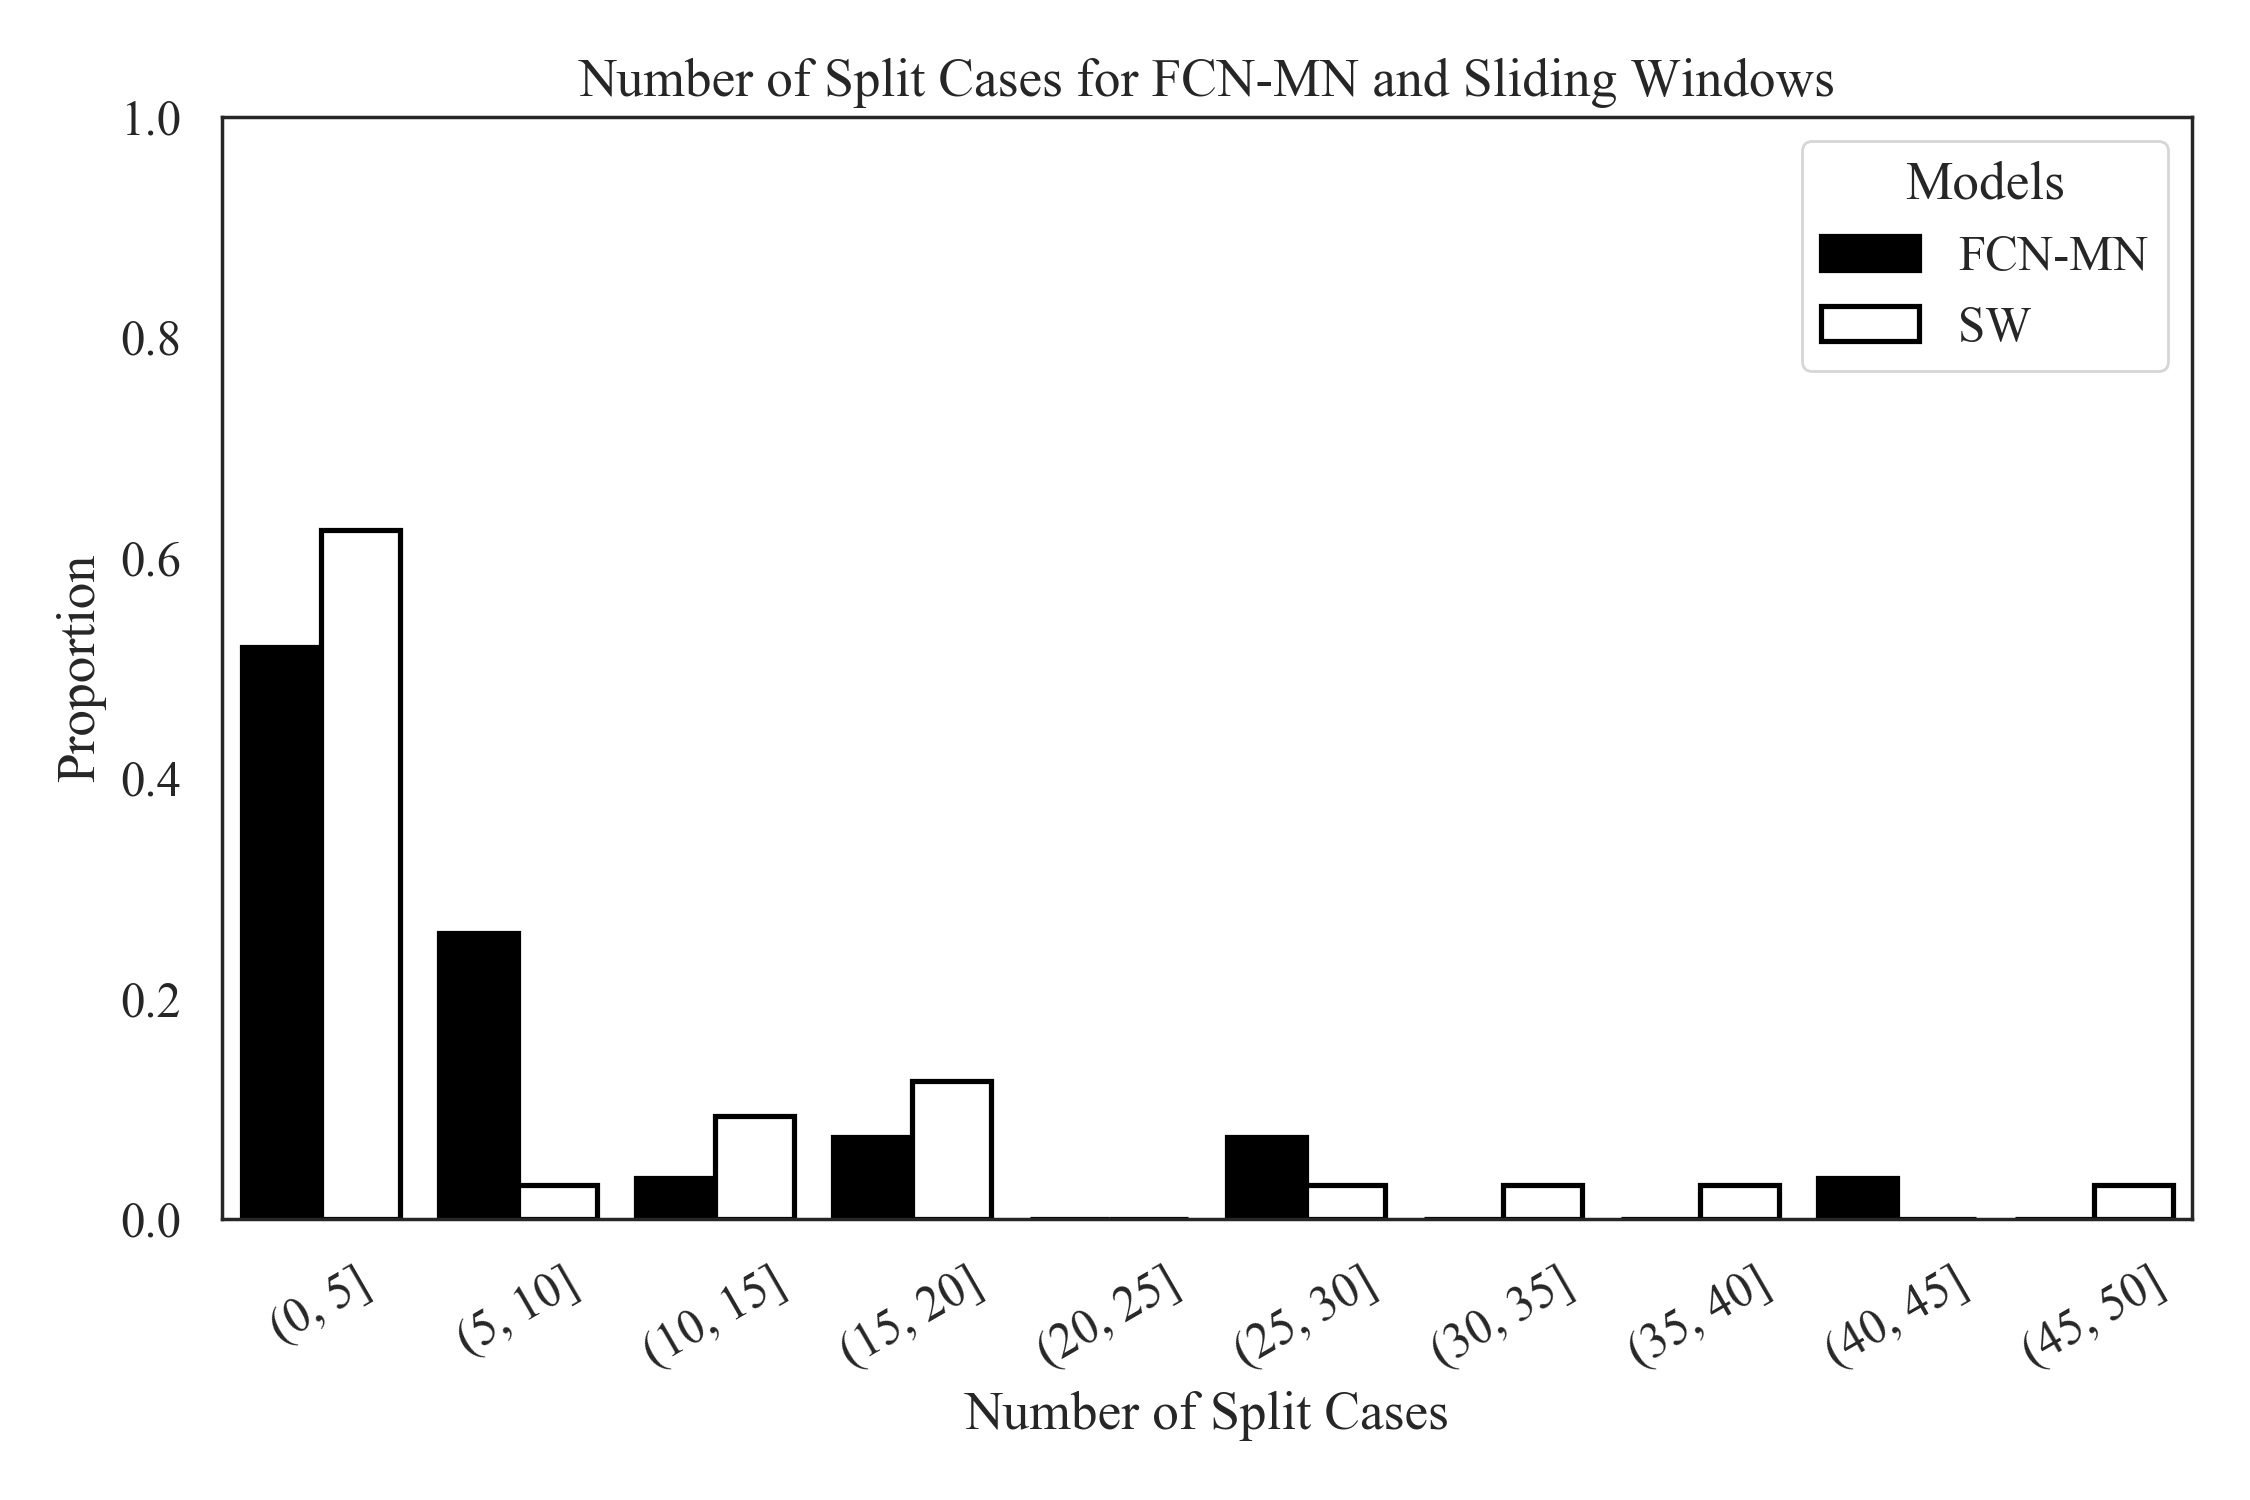
\includegraphics[width=\textwidth]{figures/PPP_split_distribution.png}
    \caption{Histogram reporting the distribution of $S$ for FCN-MN and SW in black and white bars, respectively. Each bar represents the proportion among all models ($27$ for FCN-MN  and $40$ for SW) that contains the number of splits indicated by the bin’s label. For instance, the first (from left to right) white bar indicates that almost $14\%$ out of the $40$ SW models contains between $0$ to $5$ splits. }
    \label{fig:number-of-split}
\end{figure}


\subsubsection{Detailed analysis of segmentation metrics}

As for the correspondence identification metrics, we show in Figures$\sim$ \ref{fig:XXX-a} and \ref{fig:XXX-b} scatter plots for the segmentation precision and segmentation-recall, for the \emph{correct detections} and \emph{splits} cases, respectively. These correspond to their respective columns of (a non-summarized version of) Table$\sim$\ref{tab:TablaXX}, with the black and white dots representing the values of FCN-MN and SW detection models, respectively. The position of each dot in the plot corresponds to the mean segmentation-precision and mean segmentation-recall over all images in the test set, computed over the correctly detected components (splitted components, respectively) of the masks produced by the detection model associated to that dot. The standard deviation of the recall (precision) is shown as a horizontal (vertical) bar.
%
In Figure$\sim$\ref{fig:XXX-a} (correctly detected), one can observe that all black dots (FCN-MN) are clustered on the upper-right corner of the graph, enclosed by a minimum precision of approximately $0.65$ and minimum recall of approximately $0.60$; while the white dots (SW) are clustered on the lower-right corner of the graph, with maximum precisions of $0.5$ and recall ranging from approximately $0.35$ to $1.0$. Overall, both algorithms show relatively high recalls, but with FCN-MN reaching much larger precisions. We can point to the coarse detection of the SW method as the main cause for the low precision, as this is reduced when extra, false positives are present in the positive mask. 
%
In Figure$\sim$\ref{fig:XXX-b} (splits), one can observe again the overwhelming improvements of FCN-MN over SW, with all (but one) SW cases presenting precisions under $60\%$, with the outlier showing a precision of nearly  $70\%$, and a similar distribution of recall values.  


%Fig XXX. 
\begin{figure}%
    \centering
    \begin{subfigure}[b]{0.45\textwidth}
        \centering
        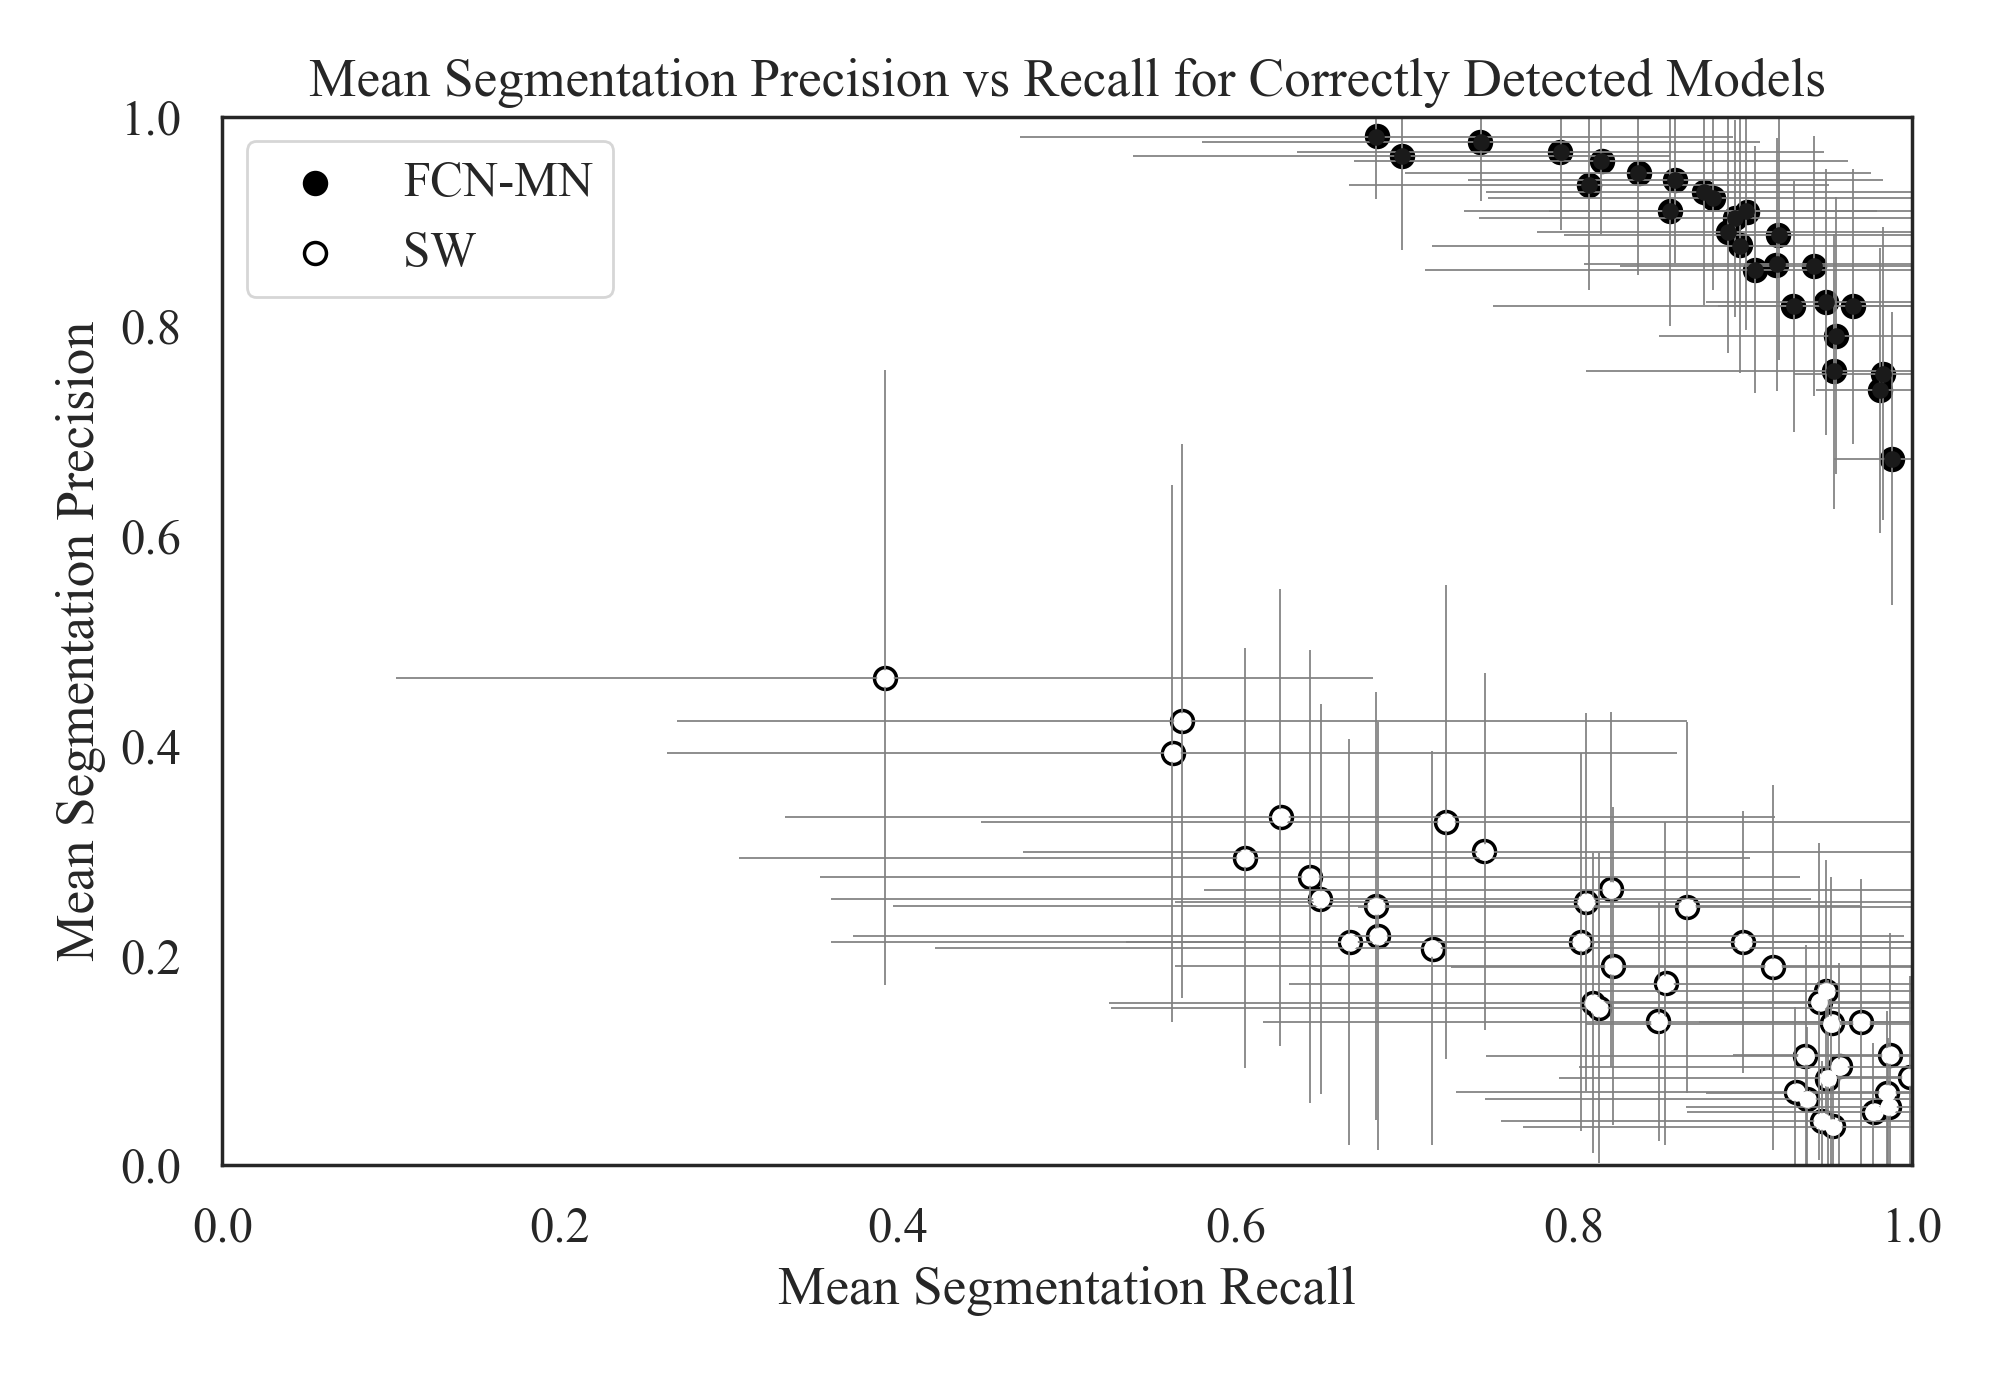
\includegraphics[width=\textwidth]{figures/XXX_correctly_detected.png}
        \caption{}
        \label{fig:XXX-a}
    \end{subfigure}
    \hfill
    \begin{subfigure}[b]{0.45\textwidth}
        \centering
        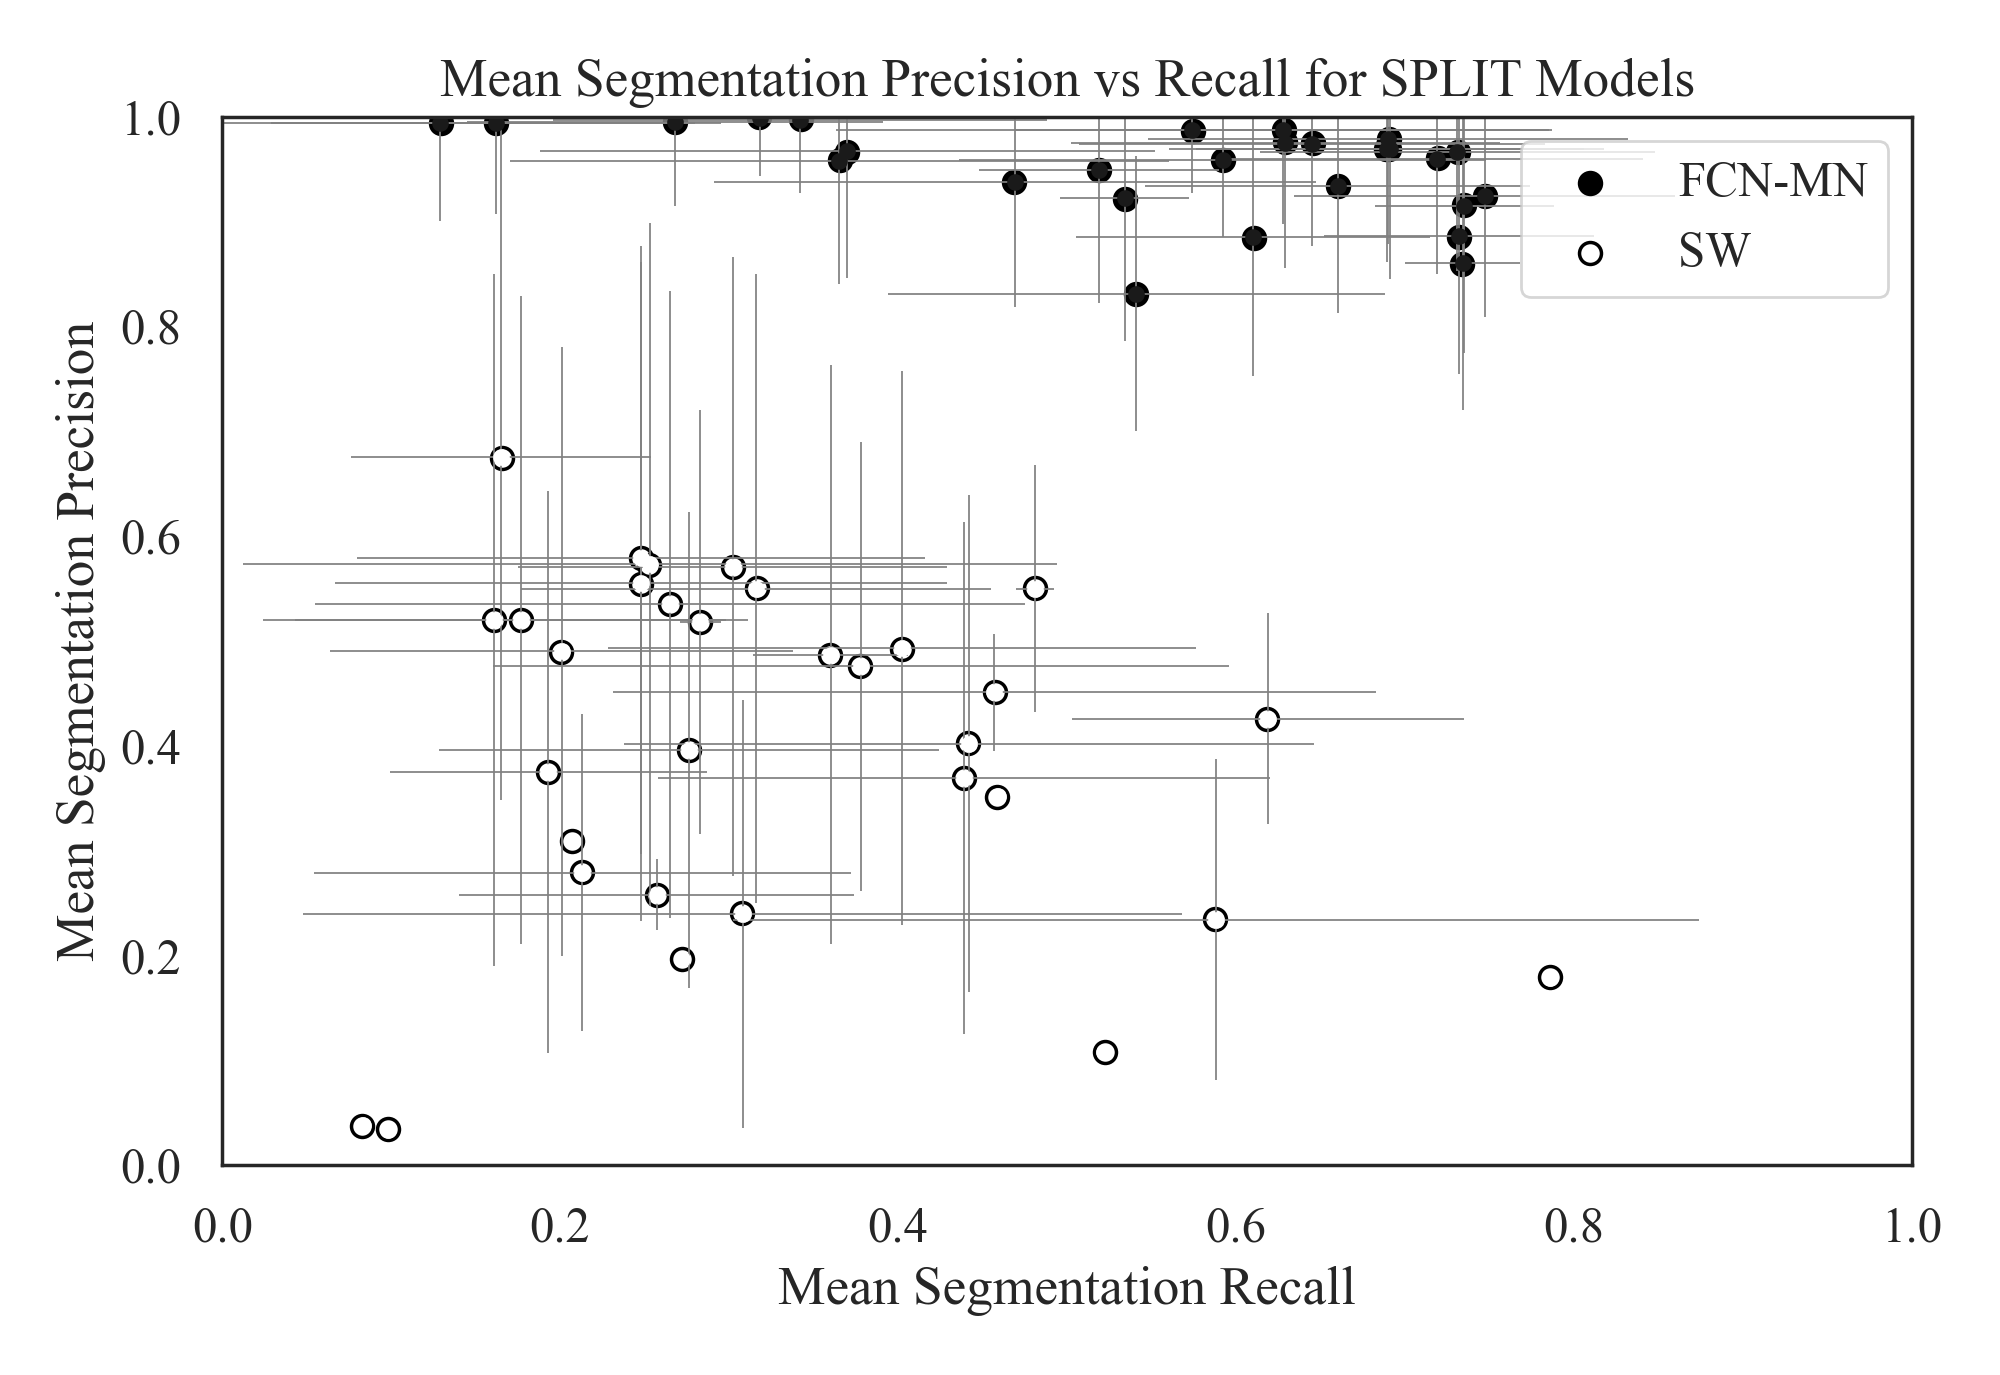
\includegraphics[width=\textwidth]{figures/XXX_splits.png}
        \caption{}
        \label{fig:XXX-b}
    \end{subfigure}
\caption{Segmentation Precision-Recall scatterplots reporting the results for FCN-MN and SW in black and white, respectively, with dots representing the average of segmentation precision and segmentation recall over all images in the test set (and bars representing standard deviations), with one dot per configuration of hyperparameters ($27$ for FCN-MN  and $40$ for SW). In (a), the averages were computed over the segmentation precision and recall of the correctly detected components, while in (b), the averages were computed  over the segmentation precision and recall of the split components.   Standar deviations.}%
    \label{fig:XXX}%
\end{figure}



%%%%%%%%%








% Figure AAA

\begin{figure}%
    \centering
      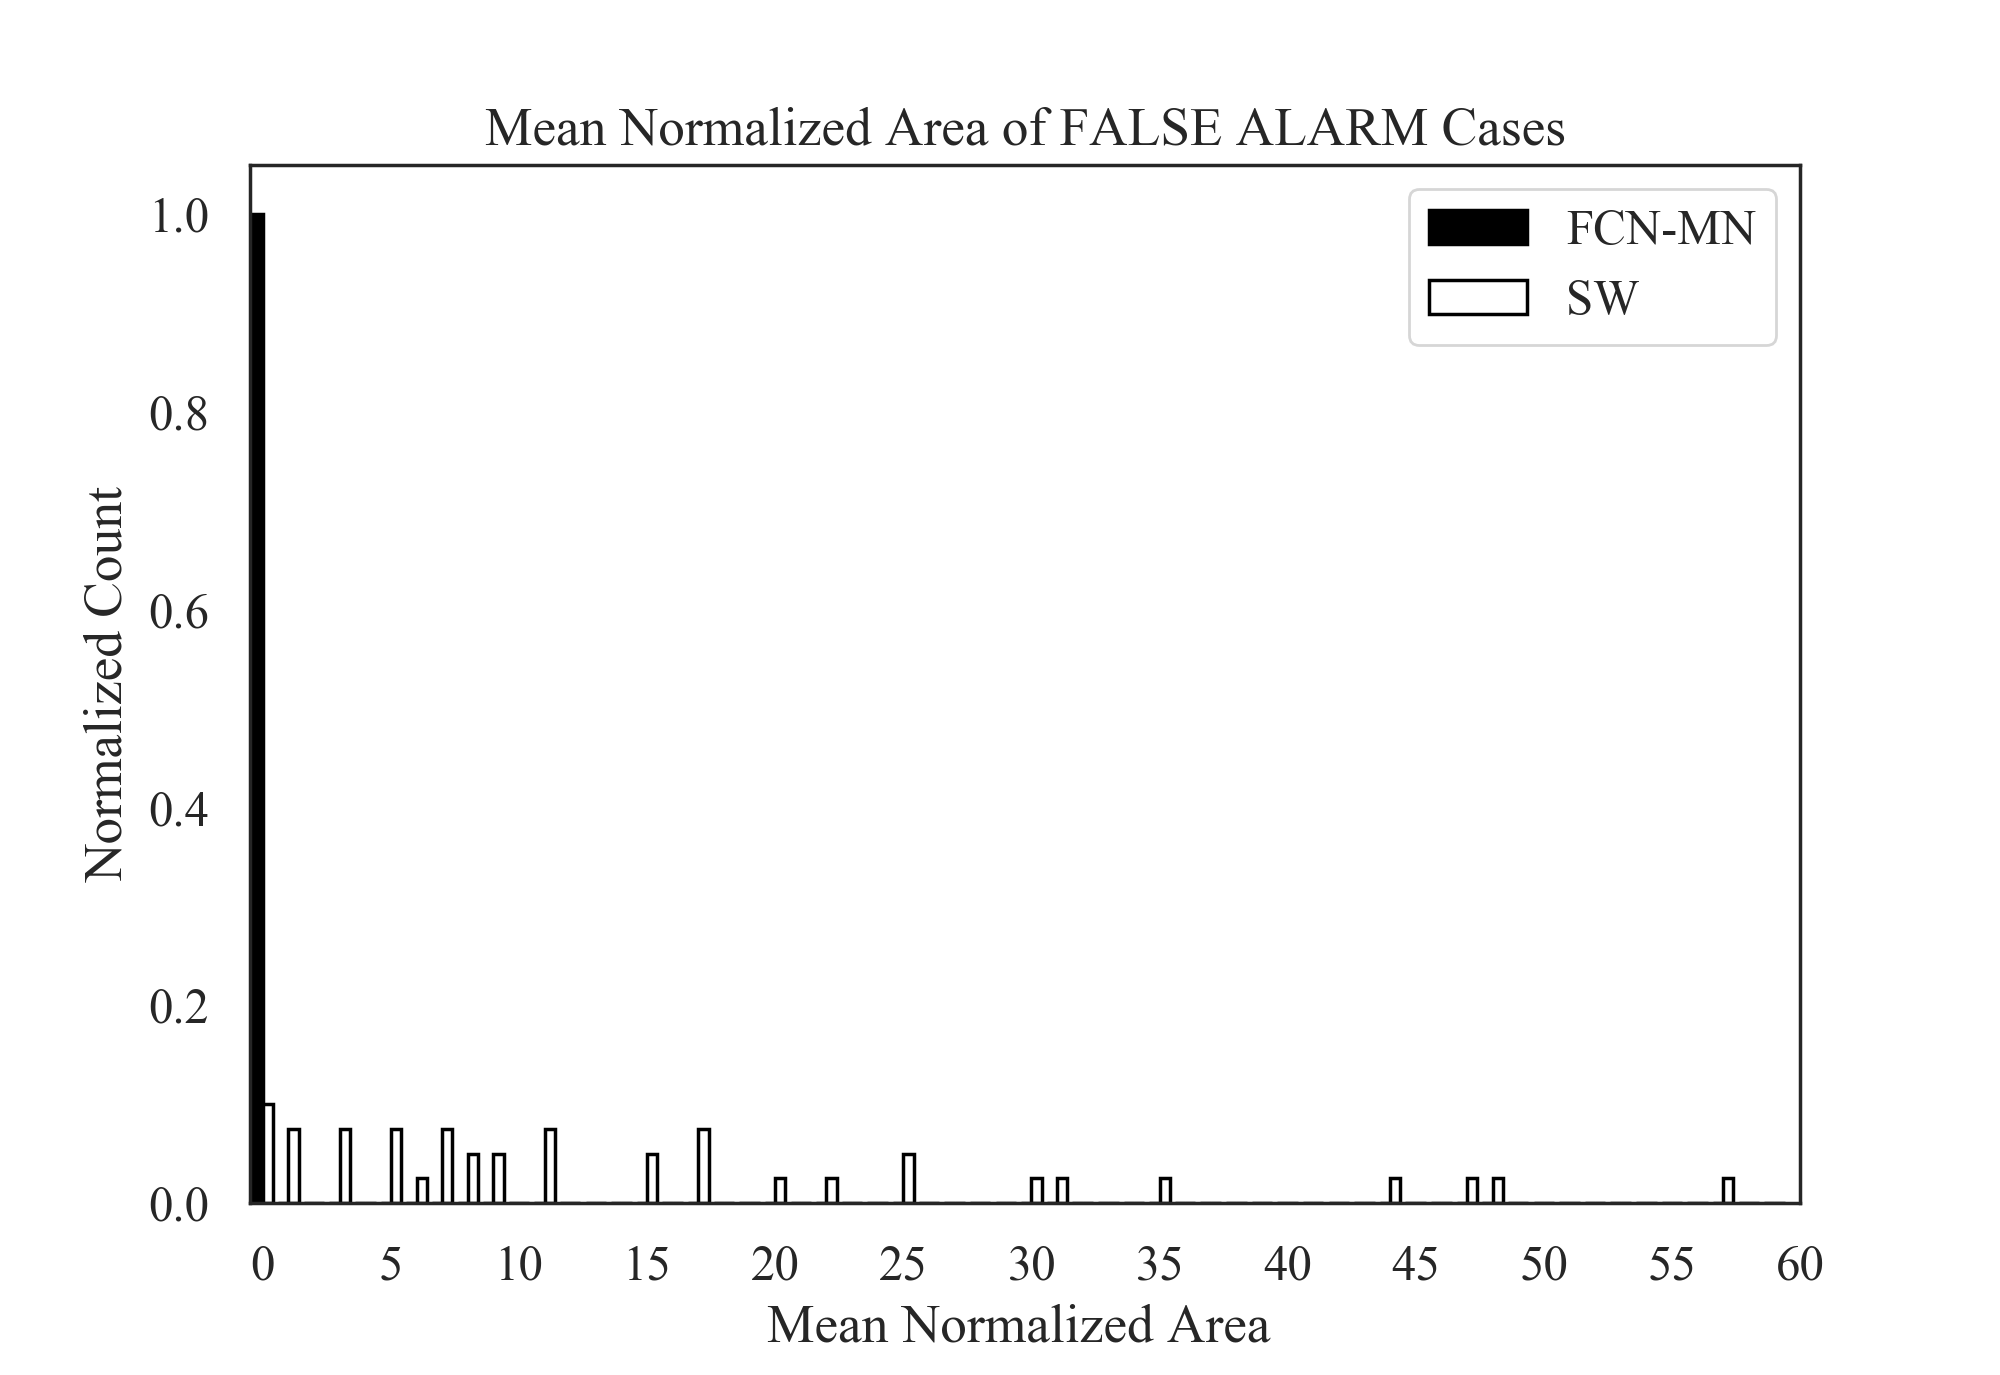
\includegraphics[width=\textwidth]{figures/AAA_mean_relative_area_fcn_vs_sw.png}%
\caption{FCN-MN (black bars) and SW (white bars) histograms of the mean normalized area $NA$ of false alarms components, with bars representing the proportion of detection models whose mean $NA$ falls within the interval of the bin.}
\label{fig:AAA}
\end{figure}

We also report graphically the segmentation results for the false alarm, the $NA$  for each of the $27$ models of FCN-MN and each of the $40$ models of SW, i.e., for each cell in the  one-before-last column of (a non-summarized version of) Table$\sim$\ref{tab:TablaXX}
%
Figure$\sim$\ref{fig:AAA} shows these results grouped in the form of two histograms, one for the FCN-MN detection models (black) and one for the SW models (in white). Bars in the histogram represent the proportion of detection models whose mean $NA$ (over all false alarm components of all images) falls within the interval of the bin. The more concentrated to the left, the better is the algorithm, as this indicates that more detection models for that algorithm resulted in smaller $NA$ (on average).
%
One can observe the histogram for FCN-MN considerably more concentrated at the left-most part of the histogram than that of SW, with all FCN-MN concentrated in a single bar at the left-most interval of  $[0.0, 1.0)$. For SW the situation is rather different, with bars at intervals as far to the right as $[57.0, 58.0)$, that is, detection models with areas as large as $58$ times the area of the bud. 
%


%%%%%%%%%%%%%%%%%%%%%%%%
\subsubsection{Detailed analysis of localization metrics}

To conclude, we present in this subsection a graphical representation of the  localization results reported in Table$\sim$\ref(tab:TablaXX), that is,  the \emph{normalized distance}($ND$) only for false alarms. This assumes that because they overlap the true bud, correctly detected and split cases should be close enough to the true bud to render it unnecessary any analysis on their distance. Instead, a false alarm can be arbitrarily far from the true bud. 

%
Figure$\sim$\ref{fig:AAA_ND} summarizes the $ND$ values reported in the corresponding column of the (non-summarized version) of Table$\sim$\ref(tab:TablaXX) in the form of two histograms, one for FCN-MN (black) and one for SW (white).  Bars in the histogram represent the proportion of detection models ($27$ for FCN-MN and $40$ for SW) whose mean $ND$ (over all false alarm components of all images) falls within the interval of the bin. The more concentrated to the left, the better is the algorithm, as this indicates that more detection models for that algorithm resulted in smaller $ND$ (on average).

%
Here again the advantage of FCN-MN over SW is clear, with the histogram for FCN-MN more concentrated to the left-most than that of SW, with the FCN-MN histogram running from the $(0,1]$ to  the $(7,8]$ bin, whereas the SW histogram running from the $(5,6]$ towards the $(9,10]$ bin. 



\begin{figure}%
    \centering
  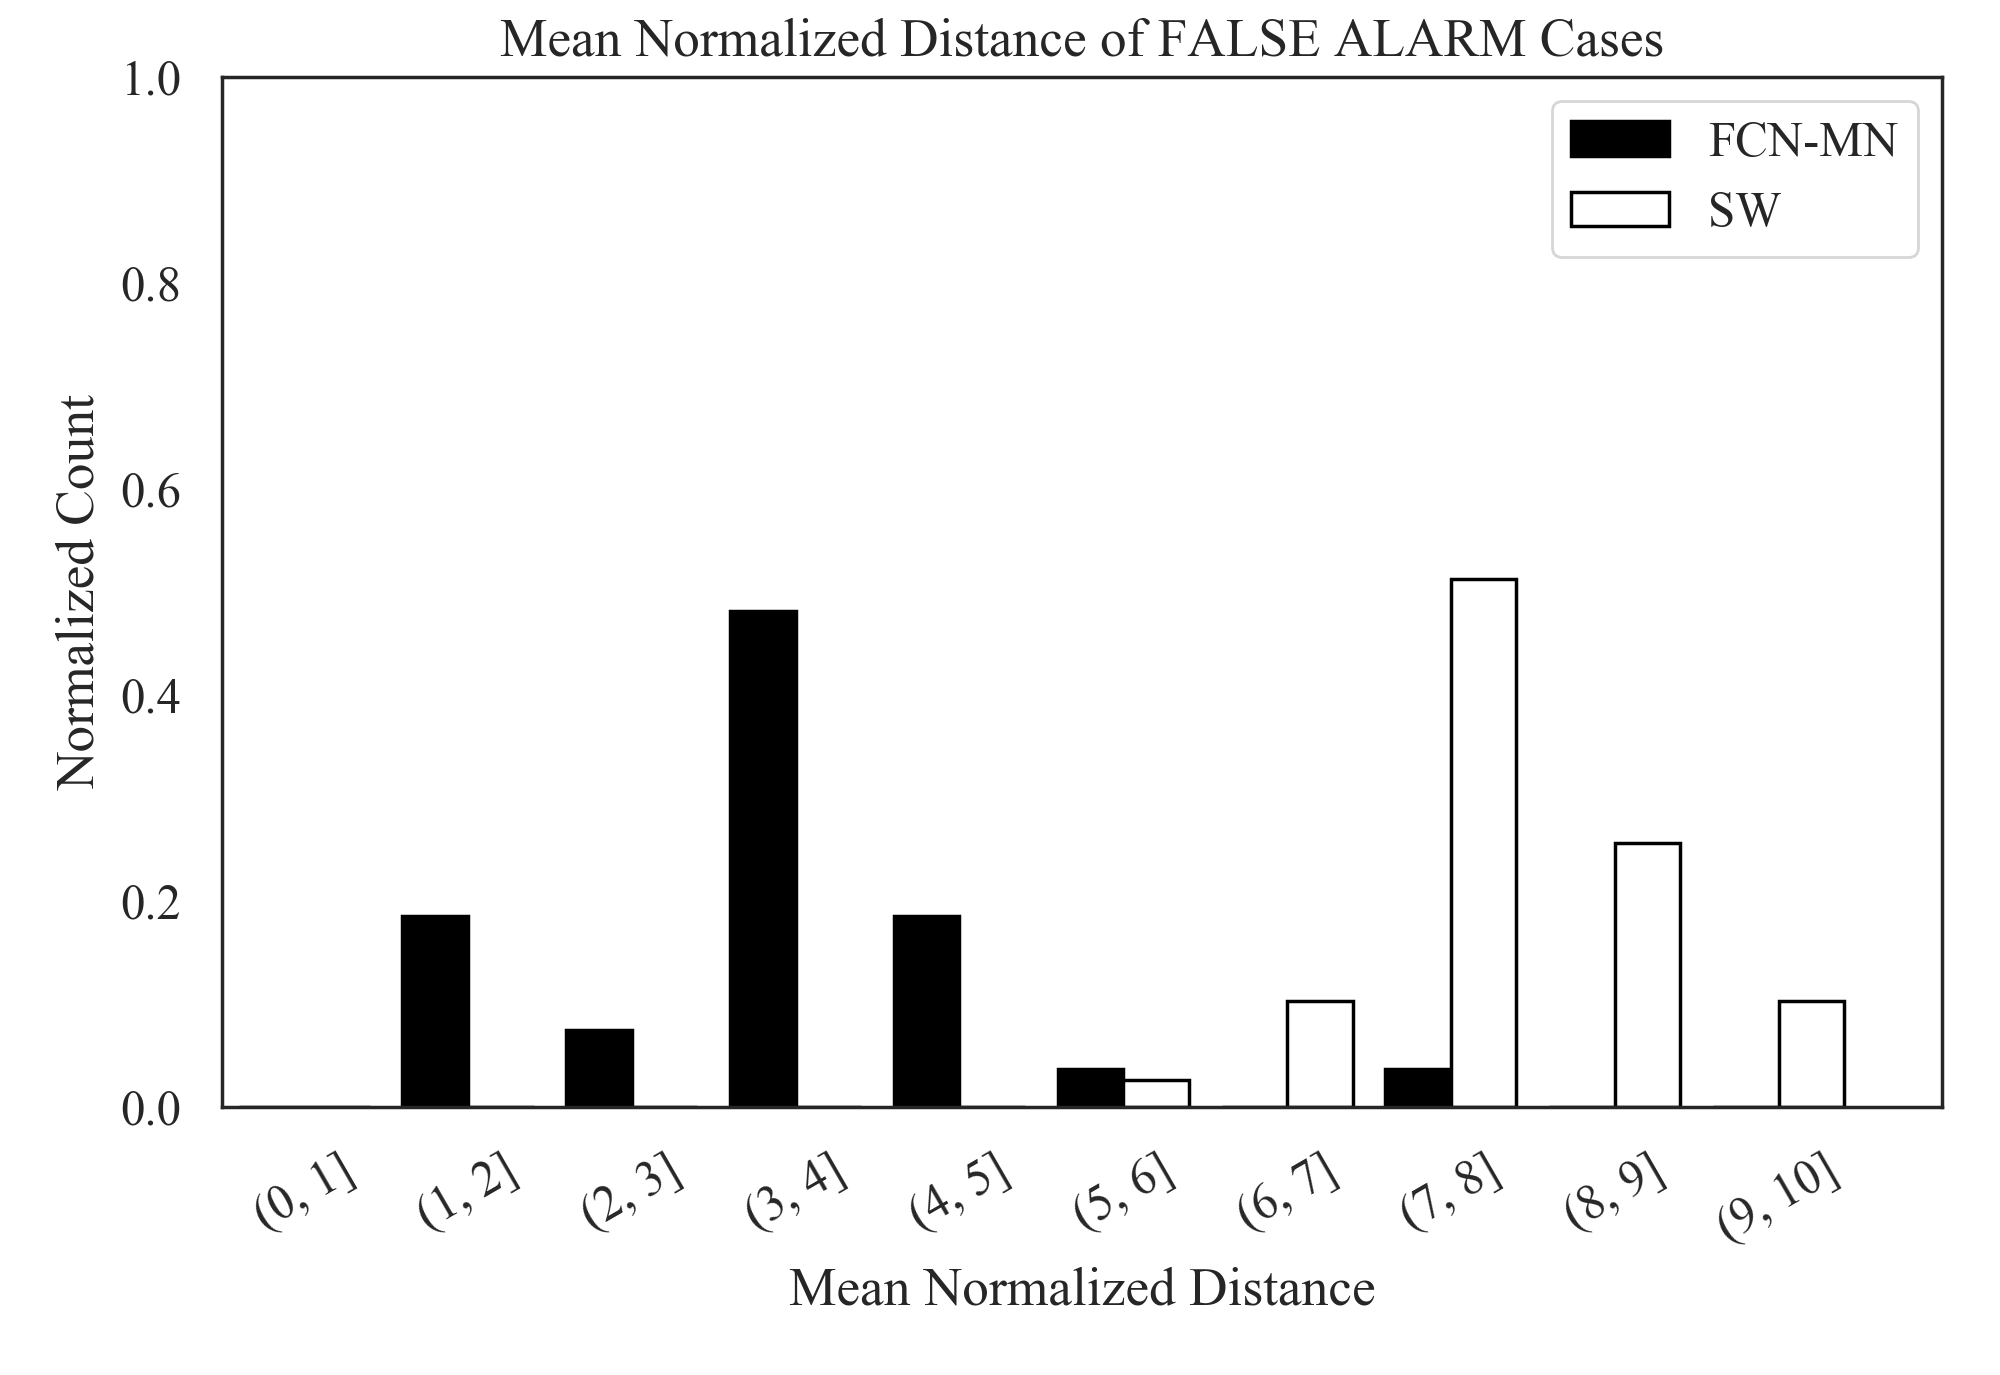
\includegraphics[width=\textwidth]{figures/AAA_normalized_distance_falsealarm_fcn_sw.png}%
\caption{FCN-MN (black bars) and SW (white bars) istograms of mean normalized distance $ND$ over all false alarms components, with bars representing the proportion of detection models whose mean $ND$ falls within the interval of the bin.}
\label{fig:AAA_ND}
\end{figure}




%#######################################################################
%#######################################################################

\section{Discussion and Conclusions} \label{sec:discussion}

%%% Presentación de la sección
En esta sección se discuten los resultados obtenidos por el enfoque propuesto en el contexto del problema de detección de yemas de vid, su impacto como herramienta para la medición de variables vitícolas de interés, y se destacan las conclusiones más importantes y presentan los trabajos futuros. 


%%% Resumen del enfoque y resultado principal (CONCLUSION)
This work introduces FCN-MN, a fully convolutional network with Mobile Net architecture for the detection of grapevine buds in 2D images captured in natural field conditions, in winter (i.e., with no leafs nor bunches), and containing a maximum of one bud.
%
The experimental results confirmed our main hypothesis, that the detection quality achieved by FCN-MN improves over the \emph{sliding windows} detector (SW) in all three detection aspects: segmentation, correspondence identification and localization. Being SW the best bud detector known to these authors, one can conclude that FCN-MN is a strong contender in the state-of-the-art for bud detectors.


% Ok, tenemos el mejor detector de yemas del mundo, pero ¿alcanza?
% ¿Alcanza para medicion de variables?

%%% Análisis caso concreto FCN-16s-0.6 
%Resaltar problemas para medir ciertas variables en 2D (e.g., distancia entre nudos, sun exposure)

But even improving over the state-of-the-art bud detectors one can still wonder if it can address the main \emph{quality} requirements of a practical measurement of the bud related variables of Table$\sim$\ref{tab:Tabla1}.

Quality performance could be assessed by the metrics reported in  Table$\sim$\ref{tab:TablaXX}, where in the best case FCN-MN shows a  detection-precision and detection-recall of $97.7$ and $100$, respectively, a mean (and standard deviation) segmentation-precision and segmentation-recall for correctly detected of $98.1(0.6)$ and $98.8(3.4)$, respectively; and for splits $99.9(0.1)$ and $74.7(28.1)$, respectively. Also, for false alarms, a maximum  $NA$ of $0.04(0.09)$ a maximum $ND$ of $0.04 (0.22)$.  
%
However, these maximums correspond each to different FCN-MN detectors. A better assessment must be conducted for one single detector. For that, we picked FCN-MN$_{16s}^{0.6}$ for showing balanced quality overall. This detector reaches detection precision and recall of $95.6$ and $93.6$ respectively, meaning than only $4.4\%$ of all the detected connected components over all test images are false alarms, and that only $6.4\%$ of all true buds could not be detected (i.e., resulted in detection failure).
%
Also, $S=3$, meaning only $3$ of all detections were splitted, which on average has a segmentation precision of $99.4(0.6)$ and segmentation recall of $16.2(10.6)$. The recall is rather small, suggesting that the split is in fact the result of pixel wise detection of the bud so sparse that it got disconnected. In contrast, all remaining detections were correct (i.e., not splitted), reaching segmentation precisions of $92.2(8.7)$, a rather similar value to that of splits, but a much larger mean segmentation recall of $88.2(13.3)$. Overall, this resulted in a mean Dice measure for the correctly detected of $89.1(10.7)$; demonstrating a considerable (mean) coverage of the true bud, with only $11.8\%$ of the buds pixels missing (on average), and only $7.8\%$ of the detected pixels covering the background (on average).
%
But more promising are the false alarm results, with $NA=0.08$ and $ND=1.1$, showing that these components are rather small, covering only an area that is $8\%$ in size of the total area of a bud (on average), and distant to the true bud by only $1.1 (0.65)$ diameters.

Based on these results, ¿what quality one should expect when the FCN-MN$_{16s}^{0.6}$ detector takes part in the measurement of the bud related variables? For brevity we discuss this  for three variables from Table$\sim$\ref{tab:Tabla1}: \emph{buds number}, \emph{bud area}, and \emph{internode length}.

 
%%% Discusión de estos resultados sobre las variables de la tabla 1
%
El caso de \emph{buds number}, por ejemplo, requiere to identify correspondences para las yemas de la escena, por lo que su calidad se verá impactada sólo por la métricas de detection precision and recall ($95.6$ and $93.6$ respectively). Para evaluar este impacto asumimos que una planta tiene aproximadamente en promedio 240 yemas. El número de yemas por planta depende de muchos factores, como ser sistema de conducción, varietal, tipo de tratamiento, época del año, entre otros, por lo que este valor se define a modo indicativo para lograr un análisis aproximado. Para este caso, una detection precision de $95.6$ resultaría en 11 yemas contadas en exceso por planta; mientras que la recall de $93.6$ resultaría en la omisión del conteo de 15 yemas. 
%
Además, este modelo produce 3 splits con dos componentes cada uno, i.e. un error de conteo por exceso del $3\%$ sobre las 140 yemas del testset. Particularmente en este análisis significa que se contarían $6$ nuevas yemas de más, dando un total de $17$ yemas en exceso, prácticamente cancelando con el error de omisión. Pero además, estos errores podrían en la práctica caracterizarse estadísticamente, permitiendo corregir las mediciones hacia valores más certeros. 
%
A pesar de estos buenos resultados, nuestro enfoque presenta aún limitaciones  prácticas para la medición del buds number debido a su imposibilidad de asociar en forma automática conteos de una misma yema en dos imágenes diferentes, dificultando  la medición masiva del conteo de las yemas de una planta o parcela. 


%
La segunda variable de interés considerada es \emph{bud area}, donde, además de identificar las correspondencias para las yemas de una escena, es necesario segmentarla para estimar su área en píxeles. El análisis de correspondence identification es análogo al del conteo de yemas, por lo que ahora se discuten sólo las métricas de segmentation. Del análisis desarrollado en los párrafos anteriores se puede concluir que los errores de segmentación por splits y false alarm tienen un bajo impacto en los resultados generales, y por ende en la estimación de \emph{bud area}. Por otro lado, si se compensan los errores de segmentación para los correct detected (i.e. $11.8\%$ of the buds pixels missing and $7.8\%$ of the detected pixels covering the background), el error de estimación del área es solo de un $4\%$. A efectos ilustrativos, vemos que este error es menor al error de precisión resultante de medir el área de una yema con un calibre. Si asumieramos que la forma de una yema se ajusta a una circunferencia, y que el diámetro típico de una yema es de $5$ mm de diámetro, obtenemos un área de $19.63 mm^2$. Siendo que un calibre tiene una precisión es $0.1 mm$, el error de precisión del área sería de $\pm 1.7 mm^2$, equivalente a un $8.6\%$ del área total; un monto que duplica el error del $4\%$ producido por nuestro detector FCN-MN. A está diferencia se le debe además sumar el error de la medición manual resultante de asumir una forma circular de la yema, aproximación innecesaria en el caso de FCN-MN.
%
Al igual que para el caso del conteo, estos buenos resultados en la precisión de la medición se ven limitados  para alcanzar un uso práctico de este tipo de medición al verse imposibilitado de asociar en forma automática mediciones de áreas de una misma yema en dos imágenes diferentes, dificultando  la medición sistemática de esta variable para las yemas de una planta o parcela. Además, en este caso, las áreas obtenidas son en píxeles, necesitando ser convertidas a magnitudes de longitud o área.


%
Por último, consideremos el caso de la \emph{internode length}, estimada por la distancia entre yemas de una misma rama (por la cercanía entre buds y nodes), la cual involucra las operaciones de correspondence identification y localización. De nuevo, el análisis de correspondence identification es análogo al del conteo de yemas, que en este caso resultará en el reporte de más de una distancia debido a la detección de más de una componente por yema. Entre estas distancias, entendemos que el peor caso puede darse entre los false alarms, siendo estos los más alejados de la true bud, y entre dos yemas ocurre cuando las false alarms están a distancia $ND$ del lado más alejado de la otra yema. En promedio, $ND = 1.1$, que de acuerdo al diámetro típico de las yemas de vid equivale a aprox. $5$mm, un valor muy menor a las distancias típicas de yemas de aproximadamente $15$cm, i.e., alrededor de un $6.6\%$ de error en la estimación de la distancia entre buds/nodes. 
%
Una limitación de nuestro enfoque para alcanzar un uso práctico de este tipo de medición es la posibilidad de determinar cuando dos yemas se encuentran en la misma rama, lo que requiere conocer la estructura de la planta.
%
Además, con nuestro método, podría medirse solamente la distancia proyectada en el plano de la imágen, la cual puede diferir arbitrariamente de la distancia real en 3D. 


% Future work for improving the results:  spatial clustering
Vemos que los errores de mayor impacto ocurren por el exceso u omisión de connected components, con el error de exceso exacerbado por el hecho de asociar buds detectadas con connected components individuales. 
%
Una mejora posible para mitigar estos errores consistiría en aplicar algunos post-procesamientos. 
%
Uno de ellos es el \emph{spatial clustering} de los connected components que los agrupe por cercanía. One could expect this to improve the results based on the small areas of split and false alarm components. On one hand, due to the closeness to the true bud of the false alarms (small $ND$), as well as the splits and  correctly detected components (they overlap with it);  and the fact that true buds in real plants are typically tens or even hundreds of bud diameters apart, a simple spatial clustering of the components would connect all these components together as one single, and correct, bud detection. Second, due to their small area, if clustered together, the false alarm components would only slightly reduce the segmentation precision.
%
Otro posible post-procesamiento consistiría en descartar connected components pequeños, por ejemplo, cuya área en pixeles normalizada respecto al área total detectada (suma de las áreas de todos los connected components) sea menor a cierto umbral. Podrían esperarse mejoras con este post-procesamiento dado que los resultados en este trabajo muestran que los false alarms presentan áreas pequeñas en relación al true bud.
% 
Por último, podrían considerarse filtros de connected components basados en la estructura de la planta, por ejemplo, descartando connected components que están lejos (o no presentan overlap) con las ramas.


% Future work for generalizing the applicability
Also, one could consider in future works some improvements that overcome the limitations for a practical use mentioned above: (i) no associations between parts of plants of different images, (ii) distance and area measurements are in pixels, (iii) only 2D geometry, (iv) lack of knowledge of the underlying plant structure, and (v) need of images with no leaves.

One could consider extending to buds the work of \cite{santos2020grape} that addresses limitation (i) for grape bunches. 
%
Limitation (ii) could be easily addressed by adding to the visual scene some marker with known dimensions. This, however, requires such a marker in every image captured, a problem that could be overcomed by first producing a calibrated 3D reconstruction of the scene, i.e., a 3D reconstruction calibrated with a single marker in one of its frames \cite{hartley2003multiple, moons20093d}. This way, every 2D image could be calibrated against the 3D model, omitting the need of a marker. 
%
In addition, a 3D reconstruction of the scene could address limitation (iii) by locating the detected buds in 3D space, following, for instance, the approach taken by \cite{diaz2018grapevine}.
%
Finally, a solution to limitations (iv) and (v) would require an integrated solution involving the detection in 3D of branches and leaves, respectively. 


%#######################################################################

\section*{Acknowledgments}

This work was funded by the National Technological University (UTN), the National Council of Scientific and Technical Research (CONICET), Argentina, and the National Fund for Scientific and Technological Promotion (FONCyT), Argentina.
%#######################################################################

%\section*{References}
\bibliography{2020-DeepBudDetection-CEA}

\end{document}
